% !Mode:: "TeX:UTF-8"
%%%%%%%%%%%%%%%%%%%%%%%%%%%%%%%%%%%%%%%%%%%%%%%%%%%%%%%%%%%%%%%%%%%%%%%%%%%%%%%%
%          ,
%      /\^/`\
%     | \/   |                CONGRATULATIONS!
%     | |    |             SPRING IS IN THE AIR!
%     \ \    /                                                _ _
%      '\\//'                                               _{ ' }_
%        ||                     hithesis v3                { `.!.` }
%        ||                                                ',_/Y\_,'
%        ||  ,                   dustincys                   {_,_}
%    |\  ||  |\          Email: yanshuoc@gmail.com             |
%    | | ||  | |            https://yanshuo.name             (\|  /)
%    | | || / /                                               \| //
%    \ \||/ /       https://github.com/dustincys/hithesis      |//
%      `\\//`   \\   \./    \\ /     //    \\./   \\   //   \\ |/ /
%     ^^^^^^^^^^^^^^^^^^^^^^^^^^^^^^^^^^^^^^^^^^^^^^^^^^^^^^^^^^^^^^
%%%%%%%%%%%%%%%%%%%%%%%%%%%%%%%%%%%%%%%%%%%%%%%%%%%%%%%%%%%%%%%%%%%%%%%%%%%%%%%%
\documentclass[fontset=fandol,type=master,campus=harbin]{hithesisbook}
% 此处选项中不要有空格
%%%%%%%%%%%%%%%%%%%%%%%%%%%%%%%%%%%%%%%%%%%%%%%%%%%%%%%%%%%%%%%%%%%%%%%%%%%%%%%%
% 必填选项
% type=doctor|master|bachelor|postdoc
%%%%%%%%%%%%%%%%%%%%%%%%%%%%%%%%%%%%%%%%%%%%%%%%%%%%%%%%%%%%%%%%%%%%%%%%%%%%%%%%
% 选填选项(选填选项的缺省值已经尽可能满足了大多数需求,除非明确知道自己有什么
% 需求)
% campus=shenzhen|weihai|harbin
%   含义:校区选项,默认harbin
% glue=true|false
%   含义:由于我工规范中要求字体行距在一个闭区间内,这个选项为true表示tex自
%   动选择,为false表示区间内一个最接近版心要求行数的要求的默认值,缺省值为
%   false。
% tocfour=true|false
%   含义:是否添加第四级目录,只对本科文科个别要求四级目录有效,缺省值为
%   false
% fontset=windows|mac|ubuntu|fandol|adobe
%   含义:设置字体,若不指定会自动识别系统,然后设置字体。fandol是开源字体,自行
%   下载安装后设置使用。windows是中易字库,窝工默认常用字体,绝对没毛病。mac和
%   ubuntu 默认分别是华文和思源字库,理论上用什么字库都行。后两种字库的安装方法
%   到谷歌上百度一下什么都有了。Linux非ubuntu发行版、非x86架构机器等如何运行可到
%   github issue上讨论。
% tocblank=true|false
%   含义:目录中第一章之前,是否加一行空白。缺省值为true。
% chapterhang=true|false
%   含义:目录的章标题是否悬挂居中,规范中要求章标题少于15字,所以这个选项
%   有无没什么用,除了特殊需求。缺省值为true。
% fulltime=true|false
%   含义:是否全日制,缺省值为true。非全日制如同等学力等,要在cover中设置类
%   型,封面中不同格式
% subtitle=true|false
%   含义:论文题目是否含有副标题,缺省值为false,如果有要在cover中设置副标
%   题内容,封面中显示。
% newgeometry=one|two|no
%   含义:规范中的自相矛盾之处,版芯是否包含页眉页脚,旧方法是按照包含页眉
%   页脚来设置。该选项是多选选项,如果设置为no,则版新为旧模板的版芯设置方法,
%   如果设置该选项one或two,分别对应两种页眉页码对应版芯线的相对位置。第一种
%   是严格按照规范要求,难看。第二种微调了页眉页码位置,好一点。默认two。
% debug=true|false
%   含义:是否显示版芯框和行号,用来调试。默认否。
% openright=true|false
%   含义:博士论文是否要求章节首页必须在奇数页,此选项不在规范要求中,按个
%   人喜好自行决定。 默认否。注意,窝工的默认情况是打印版博士论文要求右翻页
%   ,电子版要求非右翻页且无空白页。如果想DIY(或身不由己DIY)在什么地方右
%   翻页,将这个选项设置为false,然后在目标位置添加`\cleardoublepage`命令即
%   可。
% library=true|false
%   含义:是否为提交到图书馆的电子版。默认否。注意:如果设置成true,那么
%   openright选项将被强制转换为false。
% capcenterlast=true|false
%   含义:图题、表题最后一行是否居中对齐(我工规范要求居中,但不要求居中对
%   齐),此选项不在规范要求中,按个人喜好自行决定。默认否。
% subcapcenterlast=true|false
%   含义:子图图题最后一行是否居中对齐(我工规范要求居中,但不要求居中对齐
%   ),此选项不在规范要求中,按个人喜好自行决定。默认否。
% absupper=true|false
%   含义:中文目录中的英文摘要在中文目录中的大小写样式歧义,在规范中要求首
%   字母大写,在work样例中是全大写。该选项控制是否全大写。默认否。
% bsmainpagenumberline=true|false
%   含义:由于本科生论文官方模板的页码和页眉格式混乱,提供这个选项自定义设
%   置是否在正文中显示页码横线,默认显示。
% bsfrontpagenumberline=true|false
%   含义:由于本科生论文官方模板的页码和页眉格式混乱,提供这个选项自定义设
%   置是否在前文中显示页码横线,默认显示。
% bsheadrule=true|false
%   含义:由于本科生论文官方模板的页码和页眉格式混乱,提供这个选项自定义设
%   置是否显示页眉横线,默认显示。
% splitbibitem=true|false
%   含义:参考文献每一个条目内能不能断页,应广大刀客要求添加。默认否。
% newtxmath=true|false
%   含义:数学字体是否使用新罗马。默认是。
% chapterbold=true|false
%   含义:本科生章标题在目录和正文中是否加粗
% engtoc=true|false
%   含义:非博士生需要添加英文目录的,手动添加,如果是博士,此开关无效
% zijv=word|regu
%   含义:字距设置为规范规定33个字还是word中34个字。默认regu。
%%%%%%%%%%%%%%%%%%%%%%%%%%%%%%%%%%%%%%%%%%%%%%%%%%%%%%%%%%%%%%%%%%%%%%%%%%%%%%%%
\usepackage{hithesis}

\graphicspath{{figures/}}

\begin{document}
\frontmatter
% !Mode:: "TeX:UTF-8"

\hitsetup{
  %******************************
  % 注意:
  %   1. 配置里面不要出现空行
  %   2. 不需要的配置信息可以删除
  %******************************
  %
  %=====
  % 秘级
  %=====
  statesecrets={公开},
  natclassifiedindex={TM301.2},
  intclassifiedindex={62-5},
  %
  %=========
  % 中文信息
  %=========
  % ctitleone={局部多孔质气体静压},%本科生封面使用
  % ctitletwo={轴承关键技术的研究},%本科生封面使用
  ctitlecover={基于深度学习的红外图像无人机检测},%放在封面中使用,自由断行
  ctitle={基于深度学习的红外图像无人机检测},%放在原创性声明中使用
  % csubtitle={一条副标题}, %一般情况没有,可以注释掉
  cxueke={工学},
  csubject={信息与通信工程},
  caffil={电子与信息工程学院},
  cauthor={陈逸飞},
  csupervisor={吴少川教授},
  % cassosupervisor={某某某教授}, % 副指导老师
  % ccosupervisor={某某某教授}, % 联合指导老师
  % 日期自动使用当前时间,若需指定按如下方式修改:
  cdate={2022年6月},
  cstudentid={20S005075},
  cstudenttype={学术学位论文}, %非全日制教育申请学位者
  % cnumber={no9527}, %编号
  % cpositionname={哈铁西站}, %博士后站名称
  % cfinishdate={20XX年X月---20XX年X月}, %到站日期
  % csubmitdate={20XX年X月}, %出站日期
  % cstartdate={3050年9月10日}, %到站日期
  % cenddate={3090年10月10日}, %出站日期
  %(同等学力人员)、(工程硕士)、(工商管理硕士)、
  %(高级管理人员工商管理硕士)、(公共管理硕士)、(中职教师)、(高校教师)等
  %
  %
  %=========
  % 英文信息
  %=========
  etitle={UAV target detection in Infrared image},
  % esubtitle={This is the sub title},
  exueke={Engineering},
  esubject={Information and Communication Engineering},
  eaffil={\emultiline[t]{School of Electronic and Information \\  Engineering}},
  eauthor={Chen YiFei},
  esupervisor={Professor Wu Shaochuan},
  % eassosupervisor={XXX},
  % 日期自动生成,若需指定按如下方式修改:
  edate={June, 2022},
  estudenttype={Master of Art},
  %
  % 关键词用“英文逗号”分割
  ckeywords={红外目标检测, YOLOv5, 轻量化},
  ekeywords={Infrared object detection, YOLOv5, Model compression},
}

\begin{cabstract}
  目标检测是对输入图像进行相应处理后得出图像中待测目标的位置和类别的一种任务。近年来随着无人机市场和技术的发展,对无人机目标的检测和打击成为了安全领域的重要任务。而红外成像相对于可见光成像有受天气影响小等优势,因此红外图像的目标检测是目标检测中的一个重要方向,针对这一问题,本文研究提出了一种基于深度学习的红外图像无人机目标检测算法。

本文研究分析了红外图像无人机检测任务中的几个难点,如缺少公开数据集、图像信噪比低、背景复杂、已有算法定位不准、嵌入式运行效率低等,提出了具有针对性的解决方案。首先本文选择了目标检测任务中表现较好的深度学习算法YOLOv5并且和其他常用算法进行了对比,实验结果表明YOLOv5算法在红外无人机检测任务中性能优于其他已有算法。针对红外图像开源数据集较少的问题,本文自行制作了红外无人机目标数据集。针对红外图像目标边缘模糊、分辨率低、信息量小等特点,本文设计了一种通道填充的数据增强算法,提升了算法的性能。针对无人机检测任务中背景复杂的问题,本文设计了一种图像拼接的数据增强算法,提升了算法对小目标的检测能力,从而提升了算法在红外无人机数据集上的检测精度。针对小目标较多造成的算法定位不准的问题,本文改进了YOLOv5算法的目标框定位损失函数,提升了算法在红外无人机数据集上的检测精度。针对实际检测任务中的实时处理需求,本文设计了一种轻量化算法并且在嵌入式设备上进行了验证,结果表明本文提出的轻量化红外无人机目标检测算法能在嵌入式设备上基本上达到实时处理的要求。

综上,本文针对红外图像的无人机目标检测问题,研究提出了一种基于深度学习的红外无人机目标检测算法,在红外无人机数据集上相对已有算法能取得更高的检测精度,该算法的轻量化版本在嵌入式设备上验证结果表示,算法运行速度达到每秒28帧,基本可以实现实时运行。
\end{cabstract}

\begin{eabstract}
  Object detection is a task of obtaining the position and category of the object to be detected in the image after corresponding processing of the input image. In recent years, the detection and attack of UAV targets has become an important task in the security field. Compared with visible light imaging, infrared imaging has the advantage of being less affected by the weather. Therefore, the target detection of infrared images is an important direction in target detection. In response to this problem, this paper proposes a deep learning-based infrared image UAV. Object detection algorithm.

This paper studies and analyzes several difficulties in the infrared image UAV detection task, such as lack of public data sets, low image signal-to-noise ratio, complex background, inaccurate positioning of existing algorithms, low embedded operation efficiency, etc. Sexual solution. First of all, this paper selects the deep learning algorithm YOLOv5, which performs better in the target detection task, and compares it with other commonly used algorithms. The experimental results show that the performance of the YOLOv5 algorithm in the infrared UAV detection task is better than other existing algorithms. Aiming at the problem that there are few open source datasets of infrared images, this paper produced an infrared UAV target dataset by itself. Aiming at the characteristics of infrared image target edge blur, low resolution and small amount of information, this paper designs a data enhancement algorithm for channel filling. Aiming at the problem of complex background in the UAV detection task, this paper designs a data enhancement algorithm for image stitching, which improves the algorithm's ability to detect small targets, thereby improving the detection accuracy of the algorithm on the infrared UAV dataset. Aiming at the problem of inaccurate positioning of the algorithm caused by many small targets, this paper improves the target frame positioning loss function of the YOLOv5 algorithm, and improves the detection accuracy of the algorithm on the infrared UAV dataset. Aiming at the real-time processing requirements in actual detection tasks, this paper designs a lightweight algorithm and validates it on embedded devices. The results show that the proposed lightweight infrared UAV target detection algorithm can basically be used on embedded devices. meet real-time processing requirements.

In summary, this paper proposes an infrared UAV target detection algorithm based on deep learning, which can achieve higher detection accuracy than existing algorithms on the infrared UAV dataset. The lightweight version of the algorithm is used in embedded devices. The above verification results show that the algorithm runs at a speed of 28 frames per second, which can basically achieve real-time operation.
\end{eabstract}
 % 封面
\makecover
\input{front/denotation}%物理量名称表,符合规范为主,有要求添加
\tableofcontents %目录
\mainmatter
\include{body/regu}
% !Mode:: "TeX:UTF-8"

\chapter{示例文档}[Example]

这是 \hithesis\ 的示例文档,基本上覆盖了模板中所有格式的设置。建议大家在使用模
板之前,除了阅读《\hithesis\:哈尔滨工业大学学位论文模板》\footnote{即
hithesis.pdf文件},本示例文档也最好能看一看。此示例文档尽量使用到所有的排版格式
,然而对于一些不在我工规范中规定的文档,理论上是由用户自由发挥,这里不给出样例
。需要另行载入的宏包和自定义命令在文件`hithesis.sty'中有示例,这里不列举。

\section{关于数字}[Number]

按《关于出版物上数字用法的试行规定》(1987年1月1日国家语言文字工作委员会等7个单位公布),除习惯用中文数字表示的以外,一般数字均用阿拉伯数字。
(1)公历的世纪、年代、年、月、日和时刻一律用阿拉伯数字,如20世纪,80年代,4时3刻等。年号要用四位数,如1989年,不能用89年。
(2)记数与计算(含正负整数、分数、小数、百分比、约数等)一律用阿拉伯数字,如3/4,4.5%,10个月,500多种等。
(3)一个数值的书写形式要照顾到上下文。不是出现在一组表示科学计量和具有统计意义数字中的一位数可以用汉字,如一个人,六条意见。星期几一律用汉字,如星期六。邻近两个数字并列连用,表示概数,应该用汉字数字,数字间不用顿号隔开,如三五天,七八十种,四十五六岁,一千七八百元等。
(4)数字作为词素构成定型的词、词组、惯用语、缩略语等应当使用汉字。如二倍体,三叶虫,第三世界,“七五”规划,相差十万八千里等。
(5)5位以上的数字,尾数零多的,可改写为以万、亿为单位的数。一般情况下不得以十、百、千、十万、百万、千万、十亿、百亿、千亿作为单位。如~\num{345000000}~公里可改写为3.45亿公里或~\num{34500}~万公里,但不能写为3亿~\num{4500}~万公里或3亿4千5百万公里。
(6)数字的书写不必每格一个数码,一般每两数码占一格,数字间分节不用分位号“,”,凡4位或4位以上的数都从个位起每3位数空半个数码(1/4汉字)。“\num{3000000}”,不要写成“3,000,000”,小数点后的数从小数点起向右按每三位一组分节。一个用阿拉伯数字书写的多位数不能从数字中间转行。
(7)数量的增加或减少要注意下列用词的概念:1)增加为(或增加到)过去的二倍,即过去为一,现在为二;2)增加(或增加了)二倍,即过去为一,现在为三;3)超额80%,即定额为100,现在为180;4)降低到80%,即过去为100,现在为80;5)降低(或降低了)80%,即原来为100,现在为20;6)为原数的1/4,即原数为4,现在为1,或原数为1,现在为0.25。
应特别注意在表达数字减小时,不宜用倍数,而应采用分数。如减少为原来的1/2,1/3等。


\section{索引示例}[Index]

为便于检索文中内容,可编制索引置于论文之后(根据需要决定是否设置)。索引以论文中
的专业词语为检索线索,指出其相关内容的所在页码。索引用中、英两种文字书写,中文在
前。\sindex[china]{qi!乔峰}\sindex[english]{Xu Zhu}\sindex[english]{Qiao Feng}
中文按各词汉语拼音第一个字母排序,英文按该词第一个英文字母排序。

\section{术语排版举例}[Glossaries and index]

术语的定义和使用可以结合索引,灵活使用。
例如,\gtssbp 是一种应用于狄利克雷过程抽样的算法。
下次出现将是另一种格式:\gtssbp 。
还可以切换单复数例如:\gscnas ,下次出现为:\gscnas 。
此处体现了\LaTeX\ 格式内容分离的优势。

\section{引用}[Cite]

\sindex[china]{du!段誉}引文标注遵照GB/T7714-2005,采用顺序编码制。正文中引用文献的标示应置于所引内容最后一个字的右上角,所引文献编号用阿拉伯数字置于方括号“[ ]”中,用小4号字体的上角标。要求:

(1)引用单篇文献时,如“二次铣削\cite{cnproceed}”。

(2)同一处引用多篇文献时,各篇文献的序号在方括号内全部列出,各序号间用“,”,如
遇连续序号,可标注讫序号。如,…形成了多种数学模型\cite{cnarticle,cnproceed}…
注意此处添加\cs{inlinecite}中文空格\inlinecite{cnarticle,cnproceed},可以在cfg文件中修改空格类型。

(3)多次引用同一文献时,在文献序号的“[ ]”后标注引文页码。如,…间质细胞CAMP含量
测定\cite[100-197]{cnarticle}…。…含量测定方法规定
\cite[92]{cnarticle}…。

(4)当提及的参考文献为文中直接说明时,则用小4号字与正文排齐,如“由文献\inlinecite{hithesis2017}可知”

\section{定理和定义等}[Theorem]
\begin{theorem}[\cite{cnproceed}]
宇宙大爆炸是一种爆炸。
\end{theorem}
\begin{definition}[(霍金)]
宇宙大爆炸是一种爆炸。
\end{definition}
\begin{assumption}
宇宙大爆炸是一种爆炸。
\end{assumption}
\begin{lemma}
宇宙大爆炸是一种爆炸。
\end{lemma}
\begin{corollary}
宇宙大爆炸是一种爆炸。
\end{corollary}
\begin{exercise}
宇宙大爆炸是一种爆炸。
\end{exercise}
\begin{problem}[(Albert Einstein)]
宇宙大爆炸是一种爆炸。
\end{problem}
\begin{remark}
宇宙大爆炸是一种爆炸。
\end{remark}
\begin{axiom}[(爱因斯坦)]
宇宙大爆炸是一种爆炸。
\end{axiom}
\begin{conjecture}
宇宙大爆炸是一种爆炸。
\end{conjecture}
\section{图片}[Pictures]
图应有自明性。插图应与文字紧密配合,文图相符,内容正确。选图要力求精练,插图、照
片应完整清晰。机械工程图:采用第一角投影法,严格按照GB4457~GB131-83《机械制图》
标准规定。数据流程图、程序流程图、系统流程图等按GB1526-89标准规定。电气图:图形
符号、文字符号等应符合附录3所列有关标准的规定。流程图:必须采用结构化程序并正确
运用流程框图。对无规定符号的图形应采用该行业的常用画法。坐标图的坐标线均用细实线
,粗细不得超过图中曲线;有数字标注的坐标图,必须注明坐标单位。照片图要求主题和主
要显示部分的轮廓鲜明,便于制版。如用放大或缩小的复制品,必须清晰,反差适中。照片
上应有表示目的物尺寸的标度。引用文献中的图时,除在正文文字中标注参考文献序号以外
,还必须在中、英文表题的右上角标注参考文献序号。

\subsection{博士毕业论文双语题注}[Doctoral picture example]
\begin{figure}[htpb]
\centering
\includegraphics[width = 0.4\textwidth]{golfer}
\bicaption[golfer1]{}{打高尔夫球球的人(博士论文双语题注)}{Fig.$\!$}{The person playing golf (Doctoral thesis)}
\end{figure}

每个图均应有图题(由图序和图名组成),图题不宜有标点符号,图名在图序之后空1个半
角字符排写。图序按章编排,如第1章第一个插图的图号为“图1-1”。图题置于图下,硕士论
文只用中文,博士论文用中、英两种文字,居中书写,中文在上,要求中文用宋体5号字,
英文用Times New Roman 5号字。有图注或其它说明时应置于图题之上。引用图应注明出处
,在图题右上角加引用文献号。图中若有分图时,分图题置于分图之下或图题之下,可以只
用中文书写,分图号用a)、b)等表示。图中各部分说明应采用中文(引用的外文图除外)或
数字符号,各项文字说明置于图题之上(有分图时,置于分图题之上)。图中文字用宋体、
Times New Roman字体,字号尽量采用5号字(当字数较多时可用小5号字,以清晰表达为原
则,但在一个插图内字号要统一)。同一图内使用文字应统一。图表中物理量、符号用斜体
。
\subsection{本硕论文题注}[Other picture example]
\begin{figure}[h]
\centering
\includegraphics[width = 0.4\textwidth]{golfer}
\caption{打高尔夫球的人,硕士论文要求只用汉语}
\end{figure}


\begin{figure}[h]
\centering
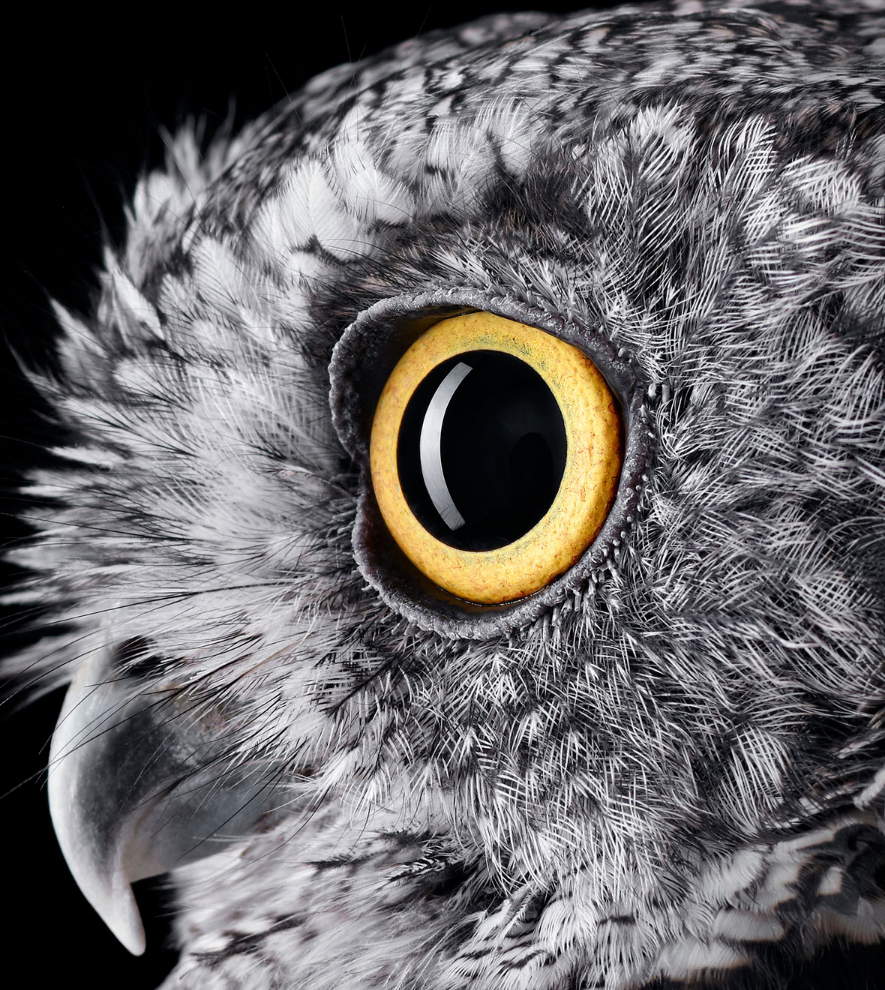
\includegraphics[width = 0.4\textwidth]{eyes.png}
\caption{眼睛}
\end{figure}

\subsection{并排图和子图}[Abreast-picture and Sub-picture example]
\subsubsection{并排图}[Abreast-picture example]

使用并排图时,需要注意对齐方式。默认情况是中部对齐。这里给出中部对齐、顶部对齐
、图片底部对齐三种常见方式。其中,底部对齐方式有一个很巧妙的方式,将长度比较小
的图放在左面即可。

\begin{figure}[htbp]
\centering
\begin{minipage}{0.4\textwidth}
\centering
\includegraphics[width=\textwidth]{golfer}
\bicaption[golfer2]{}{打高尔夫球的人}{Fig.$\!$}{The person playing golf}
\end{minipage}
\centering
\begin{minipage}{0.4\textwidth}
\centering
\includegraphics[width=\textwidth]{golfer}
\bicaption[golfer3]{}{打高尔夫球的人。注意,这里默认居中}{Fig.$\!$}{The person playing golf. Please note that, it is vertically center aligned by default.}
\end{minipage}
\end{figure}

\begin{figure}[htbp]
\centering
\begin{minipage}[t]{0.4\textwidth}
\centering
\includegraphics[width=\textwidth]{golfer}
\bicaption[golfer5]{}{打高尔夫球的人}{Fig.$\!$}{The person playing golf}
\end{minipage}
\centering
\begin{minipage}[t]{0.4\textwidth}
\centering
\includegraphics[width=\textwidth]{golfer}
\bicaption[golfer8]{}{打高尔夫球的人。注意,此图是顶部对齐}{Fig.$\!$}{The person playing golf. Please note that, it is vertically top aligned.}
\end{minipage}
\end{figure}

\begin{figure}[htbp]
\centering
\begin{minipage}[t]{0.4\textwidth}
\centering
\includegraphics[width=\textwidth,height=\textwidth]{golfer}
\bicaption[golfer9]{}{打高尔夫球的人。注意,此图对齐方式是图片底部对齐}{Fig.$\!$}{The person playing golf. Please note that, it is vertically bottom aligned for figure.}
\end{minipage}
\centering
\begin{minipage}[t]{0.4\textwidth}
\centering
\includegraphics[width=\textwidth]{golfer}
\bicaption[golfer6]{}{打高尔夫球的人}{Fig.$\!$}{The person playing golf}
\end{minipage}
\end{figure}

\subsubsection{子图}[Sub-picture example]
注意:子图题注也可以只用中文。规范规定“分图题置于分图之下或图题之下”,但没有给出具体的格式要求。
没有要求的另外一个说法就是“无论什么格式都不对”。
所以只有在一个图中有标注“a),b)”,无法使用\cs{subfigure}的情况下,使用最后一个图例中的格式设置方法,否则不要使用。
为了应对“无论什么格式都不对”,这个子图图题使用“minipage”和“description”环境,宽度,对齐方式可以按照个人喜好自由设置,是否使用双语子图图题也可以自由设置。

\begin{figure}[!h]
\setlength{\subfigcapskip}{-1bp}
\centering
\begin{minipage}{\textwidth}
\centering
\subfigure{\label{golfer41}}\addtocounter{subfigure}{-2}
\subfigure[The person playing golf]{\subfigure[打高尔夫球的人~1]{\includegraphics[width=0.4\textwidth]{golfer}}}
\hspace{2em}
\subfigure{\label{golfer42}}\addtocounter{subfigure}{-2}
\subfigure[The person playing golf]{\subfigure[打高尔夫球的人~2]{\includegraphics[width=0.4\textwidth]{golfer}}}
\end{minipage}
\centering
\begin{minipage}{\textwidth}
\centering
\subfigure{\label{golfer43}}\addtocounter{subfigure}{-2}
\subfigure[The person playing golf]{\subfigure[打高尔夫球的人~3]{\includegraphics[width=0.4\textwidth]{golfer}}}
\hspace{2em}
\subfigure{\label{golfer44}}\addtocounter{subfigure}{-2}
\subfigure[The person playing golf. Here, 'hang indent' and 'center last line' are not stipulated in the regulation.]{\subfigure[打高尔夫球的人~4。注意,规范中没有明确规定要悬挂缩进、最后一行居中。]{\includegraphics[width=0.4\textwidth]{golfer}}}
\end{minipage}
\vspace{0.2em}
\bicaption[golfer4]{}{打高尔夫球的人}{Fig.$\!$}{The person playing gol}
\end{figure}

\begin{figure}[t]
  \centering
  \begin{minipage}{.7\linewidth}
    \setlength{\subfigcapskip}{-1bp}
    \centering
    \begin{minipage}{\textwidth}
      \centering
      \subfigure{\label{golfer45}}\addtocounter{subfigure}{-2}
      \subfigure[The person playing golf]{\subfigure[打高尔夫球的人~1]{\includegraphics[width=0.4\textwidth]{golfer}}}
      \hspace{4em}
      \subfigure{\label{golfer46}}\addtocounter{subfigure}{-2}
      \subfigure[The person playing golf]{\subfigure[打高尔夫球的人~2]{\includegraphics[width=0.4\textwidth]{golfer}}}
    \end{minipage}
    \vskip 0.2em
  \wuhao 注意:这里是中文图注添加位置(我工要求,图注在图题之上)。
    \vspace{0.2em}
\bicaption[golfer47]{}{打高尔夫球的人。注意,此处我工有另外一处要求,子图图题可以位于主图题之下。但由于没有明确说明位于下方具体是什么格式,所以这里不给出举例。}{Fig.$\!$}{The person playing golf. Please note that, although it is appropriate to put subfigures' captions under this caption as stipulated in regulation, but its format is not clearly stated.}
  \end{minipage}
\end{figure}

\begin{figure}[t]
\centering
\begin{tikzpicture}
	\node[anchor=south west,inner sep=0] (image) at (0,0) {\includegraphics[width=0.3\textwidth]{golfer}};
	\begin{scope}[x={(image.south east)},y={(image.north west)}]
		\node at (0.3,0.5) {a)};
		\node at (0.8,0.2) {b)};
	\end{scope}
\end{tikzpicture}
\bicaption[golfer0]{}{打高尔夫球球的人(博士论文双语题注)}{Fig.$\!$}{The person playing golf (Doctoral thesis)}
\vskip -0.4em
 \hspace{2em}
\begin{minipage}[t]{0.3\textwidth}
\wuhao \setlist[description]{font=\normalfont}
	\begin{description}
		\item[(a)]子图图题
	\end{description}
 \end{minipage}
 \hspace{2em}
 \begin{minipage}[t]{0.3\textwidth}
\wuhao \setlist[description]{font=\normalfont}
	\begin{description}
		\item[(b)]子图图题
		\item[(b)]Subfigure caption
	\end{description}
\end{minipage}
\end{figure}


\begin{figure}[!h]
	\centering
	\begin{sideways}
		\begin{minipage}{\textheight}
			\centering
			\fbox{\includegraphics[width=0.2\textwidth]{golfer}}
			\fbox{\includegraphics[width=0.2\textwidth]{golfer}}
			\fbox{\includegraphics[width=0.2\textwidth]{golfer}}
			\fbox{\includegraphics[width=0.2\textwidth]{golfer}}
			\fbox{\includegraphics[width=0.2\textwidth]{golfer}}
			\fbox{\includegraphics[width=0.2\textwidth]{golfer}}
			\fbox{\includegraphics[width=0.2\textwidth]{golfer}}
\bicaption[golfer7]{}{打高尔夫球的人(非规范要求)}{Fig.$\!$}{The person playing golf (Not stated in the regulation)}
		\end{minipage}
	\end{sideways}
\end{figure}

\clearpage

如果不想让图片浮动到下一章节,那么在此处使用\cs{clearpage}命令。

\section{如何做出符合规范的漂亮的图}
关于作图工具在后文\ref{drawtool}中给出一些作图工具的介绍,此处不多言。
此处以R语言和Tikz为例说明如何做出符合规范的图。

\subsection{Tikz作图举例}
使用Tikz作图核心思想是把格式、主题、样式与内容分离,定义在全局中。
注意字体设置可以有两种选择,如何字少,用五号字,字多用小五。
使用Tikz作图不会出现字体问题,字体会自动与正文一致。

\begin{figure}[thb!]
  \centering
      \begin{tikzpicture}[xscale=0.8,yscale=0.3,rotate=90]
        \small
	\draw (-22,6.5) node[refcell]{参考基因组};
	\draw[refline] (-23, 5) -- (27, 5);
	\draw (-22,3.75) node[tscell]{肿瘤样本};
	\draw (-20,3.75) node[tncell]{正常细胞};
	\draw[tnline] (-21, 2.5) -- (27, 2.5);
	\draw (-20,1.25) node[ttcell]{肿瘤细胞};
	\rcell{2}{6};
	\draw[fakeevolve] (4.5, 5.25) -- (4.5, 4.8);
	\ncell{2}{4};
	\draw[evolve] (4.5, 3) .. controls (4.5,2.8) and (-3.5,2.9) ..  (-3.5, 2);
	\draw[evolve] (4.5, 3) .. controls (4.5,2.8) and (11.5,2.9) .. (11.5, 2);
	\tcellone{-6}{1.5};
	\draw (-9, 2) node[ttcell]{1};
	\draw[evolve] (-3.5, 0) .. controls (-3.5,-0.2) and (-12,-0.1) .. (-12, -1.5);
	\draw[evolve] (-3.5, 0) .. controls (-3.5,-0.2) and (1.5,-0.1) .. (1.5, -1.5);
	\tcellthree{7}{1.5};
	\draw (4, 2) node[ttcell]{2};
	\draw[evolve] (11, 0.5) .. controls (11,0.3) and (19,0.4) .. (19, -1.5);
	\tcellfive{-16}{-2};
	\draw (-19, -1.5) node[ttcell]{3};
	\tcelltwo{-1}{-2};
	\draw (-4, -1.5) node[ttcell]{4};
	\tcellfour{12}{-2};
	\draw (9, -1.5) node[ttcell]{5};
      \end{tikzpicture}
  \begin{minipage}{.9\linewidth}
      \vskip 0.2em
      \wuhao 图中,带有箭头的淡蓝色箭头表示肿瘤子种群的进化方向。一般地,从肿瘤组织中取用于进行二代测序的样本中含有一定程度的正常细胞污染,因此肿瘤的样本中含有正常细胞和肿瘤细胞。每一个子种群的基因组的模拟过程是把生殖细胞变异和体细胞变异加入到参考基因组中。
      \vspace{0.6em}
  \end{minipage}
\bicaption[tumor]{}{肿瘤组织中各个子种群的进化示意图}{Fig.$\!$}{The diagram of tumor subpopulation evolution process}
\end{figure}

\subsection{R作图}
R是一种极具有代表性的典型的作图工具,应用广泛。
与Tikz图~\ref{tumor}~不同,R作图分两种情况:(1)可以转换为Tikz码;(2)不可转换为Tikz码。
第一种情况图形简单,图形中不含有很多数据点,使用R语言中的Tikz包即可。
第二种情况是图形复杂,含有海量数据点,这时候不要转成Tikz矢量图,这会使得论文体积巨大。
推荐使用pdf或png非矢量图形。
使用非矢量图形时要注意选择好字号(五号或小五),和字体(宋体、新罗马)然后选择生成图形大小,注意此时在正文中使用\cs{includegraphics}命令导入时,不要像导入矢量图那样控制图形大小,使用图形的原本的
宽度和高度,这样就确保了非矢量图形中的文字与正文一致了。

为了控制\hithesis\ 的大小,此处不给出具体举例,

\section{表格}

表应有自明性。表格不加左、右边线。表的编排建议采用国际通行的三线表。表中文字用宋
体~5~号字。每个表格均应有表题(由表序和表名组成)。表序一般按章编排,如第~1~章第
一个插表的序号为“表~1-1”等。表序与表名之间空一格,表名中不允许使用标点符号,表名
后不加标点。表题置于表上,硕士学位论文只用中文,博士学位论文用中、英文两种文字居
中排写,中文在上,要求中文用宋体~5~号字,英文用新罗马字体~5~号字。表头设计应简单
明了,尽量不用斜线。表头中可采用化学符号或物理量符号。


\subsection{普通表格的绘制方法}[Methods of drawing normal tables]

表格应具有三线表格式,因此需要调用~booktabs~宏包,其标准格式如表~\ref{table1}~所示。
\begin{table}[htbp]
\bicaption[table1]{}{符合研究生院绘图规范的表格}{Table$\!$}{Table in agreement of the standard from graduate school}
\vspace{0.5em}\centering\wuhao
\begin{tabular}{ccccc}
\toprule
$D$(in) & $P_u$(lbs) & $u_u$(in) & $\beta$ & $G_f$(psi.in)\\
\midrule
 5 & 269.8 & 0.000674 & 1.79 & 0.04089\\
10 & 421.0 & 0.001035 & 3.59 & 0.04089\\
20 & 640.2 & 0.001565 & 7.18 & 0.04089\\
\bottomrule
\end{tabular}
\end{table}
全表如用同一单位,则将单位符号移至表头右上角,加圆括号。表中数据应准确无误,书写
清楚。数字空缺的格内加横线“-”(占~2~个数字宽度)。表内文字或数字上、下或左、右
相同时,采用通栏处理方式,不允许用“〃”、“同上”之类的写法。表内文字说明,起行空一
格、转行顶格、句末不加标点。如某个表需要转页接排,在随后的各页上应重复表的编号。
编号后加“(续表)”,表题可省略。续表应重复表头。

\subsection{长表格的绘制方法}[Methods of drawing long tables]

长表格是当表格在当前页排不下而需要转页接排的情况下所采用的一种表格环境。若长表格
仍按照普通表格的绘制方法来获得,其所使用的\verb|table|浮动环境无法实现表格的换页
接排功能,表格下方过长部分会排在表格第1页的页脚以下。为了能够实现长表格的转页接
排功能,需要调用~longtable~宏包,由于长表格是跨页的文本内容,因此只需要单独的
\verb|longtable|环境,所绘制的长表格的格式如表~\ref{table2}~所示。

注意,长表格双语标题的格式。

\vspace{-1.5bp}
\ltfontsize{\wuhao[1.667]}
\wuhao[1.667]\begin{longtable}{ccc}%
\longbionenumcaption{}{{\wuhao 中国省级行政单位一览}\label{table2}}{Table$\!$}{}{{\wuhao Overview of the provincial administrative unit of China}}{-0.5em}{3.15bp}\\
%\caption{\wuhao 中国省级行政单位一览}\label{table2}\\
\toprule 名称 & 简称 & 省会或首府\\ \midrule
\endfirsthead
\multicolumn{3}{r}{表~\thetable(续表)}\vspace{0.5em}\\
\toprule 名称 & 简称 & 省会或首府\\ \midrule
\endhead
\midrule[0.5pt]
\endfoot
\bottomrule
\endlastfoot
北京市 & 京 & 北京\\
天津市 & 津 & 天津\\
河北省 & 冀 & 石家庄市\\
山西省 & 晋 & 太原市\\
内蒙古自治区 & 蒙 & 呼和浩特市\\
辽宁省 & 辽 & 沈阳市\\
吉林省 & 吉 & 长春市\\
黑龙江省 & 黑 & 哈尔滨市\\
上海市 & 沪/申 & 上海\\
江苏省 & 苏 & 南京市\\
浙江省 & 浙 & 杭州市\\
安徽省 & 皖 & 合肥市\\
福建省 & 闽 & 福州市\\
江西省 & 赣 & 南昌市\\
山东省 & 鲁 & 济南市\\
河南省 & 豫 & 郑州市\\
湖北省 & 鄂 & 武汉市\\
湖南省 & 湘 & 长沙市\\
广东省 & 粤 & 广州市\\
广西壮族自治区 & 桂 & 南宁市\\
海南省 & 琼 & 海口市\\
重庆市 & 渝 & 重庆\\
四川省 & 川/蜀 & 成都市\\
贵州省 & 黔/贵 & 贵阳市\\
云南省 & 云/滇 & 昆明市\\
西藏自治区 & 藏 & 拉萨市\\
陕西省 & 陕/秦 & 西安市\\
甘肃省 & 甘/陇 & 兰州市\\
青海省 & 青 & 西宁市\\
宁夏回族自治区 & 宁 & 银川市\\
新疆维吾尔自治区 & 新 & 乌鲁木齐市\\
香港特别行政区 & 港 & 香港\\
澳门特别行政区 & 澳 & 澳门\\
台湾省 & 台 & 台北市\\
\end{longtable}\normalsize
\vspace{-1em}

此长表格~\ref{table2}~第~2~页的标题“编号(续表)”和表头是通过代码自动添加上去的,无需人工添加,若表格在页面中的竖直位置发生了变化,长表格在第~2~页
及之后各页的标题和表头位置能够始终处于各页的最顶部,也无需人工调整,\LaTeX~系统的这一优点是~word~等软件所无法比拟的。

\subsection{列宽可调表格的绘制方法}[Methods of drawing tables with adjustable-width columns]
论文中能用到列宽可调表格的情况共有两种,一种是当插入的表格某一单元格内容过长以至
于一行放不下的情况,另一种是当对公式中首次出现的物理量符号进行注释的情况,这两种
情况都需要调用~tabularx~宏包。下面将分别对这两种情况下可调表格的绘制方法进行阐述
。
\subsubsection{表格内某单元格内容过长的情况}[The condition when the contents in
some cells of tables are too long]
首先给出这种情况下的一个例子如表~\ref{table3}~所示。
\begin{table}[htbp]
  \centering
\bicaption[table3]{}{最小的三个正整数的英文表示法}{Table$\!$}{The English construction of the smallest three positive integral numbers}\vspace{0.5em}\wuhao
\begin{tabularx}{0.7\textwidth}{llX}
\toprule
Value & Name & Alternate names, and names for sets of the given size\\
\midrule
1 & One & ace, single, singleton, unary, unit, unity\\
2 & Two & binary, brace, couple, couplet, distich, deuce, double, doubleton, duad, duality, duet, duo, dyad, pair, snake eyes, span, twain, twosome, yoke\\
3 & Three & deuce-ace, leash, set, tercet, ternary, ternion, terzetto, threesome, tierce, trey, triad, trine, trinity, trio, triplet, troika, hat-trick\\
\bottomrule
\end{tabularx}
\end{table}
tabularx环境共有两个必选参数:第1个参数用来确定表格的总宽度,第2个参数用来确定每
列格式,其中标为X的项表示该列的宽度可调,其宽度值由表格总宽度确定。标为X的列一般
选为单元格内容过长而无法置于一行的列,这样使得该列内容能够根据表格总宽度自动分行
。若列格式中存在不止一个X项,则这些标为X的列的列宽相同,因此,一般不将内容较短的
列设为X。标为X的列均为左对齐,因此其余列一般选为l(左对齐),这样可使得表格美观
,但也可以选为c或r。

\subsubsection{对物理量符号进行注释的情况}[The condition when physical symbols
need to be annotated]

为使得对公式中物理量符号注释的转行与破折号“———”后第一个字对齐,此处最好采用表格
环境。此表格无任何线条,左对齐,且在破折号处对齐,一共有“式中”二字、物理量符号和
注释三列,表格的总宽度可选为文本宽度,因此应该采用\verb|tabularx|环境。由
\verb|tabularx|环境生成的对公式中物理量符号进行注释的公式如式(\ref{eq:1})所示。
\begin{equation}\label{eq:1}
\ddot{\boldsymbol{\rho}}-\frac{\mu}{R_{t}^{3}}\left(3\mathbf{R_{t}}\frac{\mathbf{R_{t}\rho}}{R_{t}^{2}}-\boldsymbol{\rho}\right)=\mathbf{a}
\end{equation}
\begin{tabularx}{\textwidth}{@{}l@{\quad}r@{———}X@{}}
式中& $\boldsymbol{\rho}$ &追踪飞行器与目标飞行器之间的相对位置矢量;\\
&  $\boldsymbol{\ddot{\rho}}$&追踪飞行器与目标飞行器之间的相对加速度;\\
&  $\mathbf{a}$   &推力所产生的加速度;\\
&  $\mathbf{R_t}$ & 目标飞行器在惯性坐标系中的位置矢量;\\
&  $\omega_{t}$ & 目标飞行器的轨道角速度;\\
&  $\mathbf{g}$ & 重力加速度,$=\frac{\mu}{R_{t}^{3}}\left(
3\mathbf{R_{t}}\frac{\mathbf{R_{t}\rho}}{R_{t}^{2}}-\boldsymbol{\rho}\right)=\omega_{t}^{2}\frac{R_{t}}{p}\left(
3\mathbf{R_{t}}\frac{\mathbf{R_{t}\rho}}{R_{t}^{2}}-\boldsymbol{\rho}\right)$,这里~$p$~是目标飞行器的轨道半通径。
\end{tabularx}\vspace{3.15bp}
由此方法生成的注释内容应紧邻待注释公式并置于其下方,因此不能将代码放入
\verb|table|浮动环境中。但此方法不能实现自动转页接排,可能会在当前页剩余空间不够
时,全部移动到下一页而导致当前页出现很大空白。因此在需要转页处理时,还请您手动将
需要转页的代码放入一个新的\verb|tabularx|环境中,将原来的一个\verb|tabularx|环境
拆分为两个\verb|tabularx|环境。

\subsubsection{排版横版表格的举例}[An example of landscape table]

\begin{table}[p]
\centering
\begin{sideways}
\begin{minipage}{\textheight}
\bicaption[table4]{}{不在规范中规定的横版表格}{Table$\!$}{A table style which is not stated in the regulation}
\vspace{0.5em}\centering\wuhao
\begin{tabular}{ccccc}
\toprule
$D$(in) & $P_u$(lbs) & $u_u$(in) & $\beta$ & $G_f$(psi.in)\\
\midrule
 5 & 269.8 & 0.000674 & 1.79 & 0.04089\\
10 & 421.0 & 0.001035 & 3.59 & 0.04089\\
20 & 640.2 & 0.001565 & 7.18 & 0.04089\\
\bottomrule
\end{tabular}
\end{minipage}
\end{sideways}
\end{table}


\section{公式}
与正常\LaTeX\ 使用方法一致,此处略。关于公式中符号样式的定义在`hithesis.sty'有示
例。

\section{其他杂项}[Miscellaneous]

\subsection{右翻页}[Open right]

对于双面打印的论文,强制使每章的标题页出现右手边为右翻页。
规范中没有明确规定是否是右翻页打印。
模板给出了右翻页选项。
为了应对用户的个人喜好,在希望设置成右翻页的位置之前添加\cs{cleardoublepage}命令即可。

\subsection{算法}[Algorithms]
我工算法有以下几大特点。

(1)算法不在规范中要求。

(2)算法常常被使用(至少计算机学院)。

(3)格式乱,甚至出现了每个实验室的格式要求都不一样。

此处不给出示例,因为没法给,在
\href{https://github.com/dustincys/PlutoThesis}{https://github.com/dustincys/PlutoThesis}
的readme文件中有不同实验室算法要求说明。

\subsection{脚注}[Footnotes]
不在再规范\footnote{规范是指\PGR\ 和\UGR}中要求,模板默认使用清华大学的格式。

\subsection{源码}[Source code]
也不在再规范中要求。如果有需要最好使用minted包,但在编译的时候需要添加“
-shell-escape”选项且安装pygmentize软件,这些不在模板中默认载入,如果需要自行载入
。
\subsection{思源宋体}[Siyuan font]
如果要使用思源字体,需要思源字体的定义文件,此文件请到模板的开发版网址github:
\href{https://github.com/dustincys/hithesis}{https://github.com/dustincys/hithesis}
或者oschia:
\href{https://git.oschina.net/dustincys/hithesis}{https://git.oschina.net/dustincys/hithesis}
处下载。

\subsection{专业绘图工具}[Processional drawing tool]
\label{drawtool}
推荐使用tikz包,使用tikz源码绘图的好处是,图片中的字体与正文中的字体一致。具体如
何使用tikz绘图不属于模板范畴。
tikz适合用来画不需要大量实验数据支撑示意图。但R语言等专业绘图工具具有画出各种、
专业、复杂的数据图。R语言中有tikz包,能自动生成tikz码,这样tikz几乎无所不能。
对于排版有极致追求的小伙伴,可以参考
\href{http://www.texample.net/tikz/resources/}{http://www.texample.net/tikz/resources/}
中所列工具,几乎所有作图软件所作的图形都可转成tikz,然后可以自由的在tikz中修改
图中内容,定义字体等等。实现前文窝工规范中要求的图中字体的一致性的终极目标。


\subsection{术语词汇管理}[Manage glossaries]
推荐使用glossaries包管理术语、缩略语,可以自动生成首次全写,非首次缩写。

\subsection{\TeX\ 源码编辑器}[\TeX editor]
推荐:(1)付费软件Winedt;(2)免费软件kile;(3)vim或emaces或sublime等神级编
译器(需要配置)。

\subsection{\LaTeX\ 排版重要原则}[\LaTeX\ typesetting rules]
格式和内容分离是\LaTeX\ 最大优势,所有多次出现的内容、样式等等都可以定义为简单命
令、环境。这样的好处是方便修改、管理。例如,如果想要把所有的表示向量的符号由粗体
\cs{mathbf}变换到花体\cs{mathcal},只需修改该格式的命令的定义部分,不需要像MS
word那样处处修改。总而言之,使用自定义命令和环境才是正确的使用\LaTeX\ 的方式。

\section{关于捐助}
各位刀客和大侠如用的嗨,要解囊相助,请参照图~\ref{zfb}~中提示操作(二维码被矢量化后之后去
除了头像等冗余无用的部分~)。

\begin{figure}[!h]
\centering\includegraphics[width=0.4\textwidth]{zfb}
\vspace{0.2em}
\bicaption[Donation]{}{捐助,注意此处是子图只用汉语图题的形式,我工规定可以不用
英语图题}{Fig.$\!$}{Donation, please note that it is OK to use Chinese caption
only}
\end{figure}


% Local Variables:
% TeX-master: "../main"
% TeX-engine: xetex
% End:

% !Mode:: "TeX:UTF-8"

\chapter{红外无人机目标检测算法}

\section{引言}
本课题研究的红外无人机目标检测算法,主要需要解决的问题有两个。
一个是原始图像是由红外设备产生的,因此原始图片是灰度图,
不含有普通BGR图像的三个通道信息;
另一个问题是在实际的检测场景下,无人机目标在检测设备中的成像往往伴随相当复杂的背景,
本课题对算法的复杂背景下目标的检测能力要求较高。
因此本章所做的研究首先是针对本课题的红外无人机目标检测问题
建立研究必要的数据集,
之后选择一种在该数据集上性能较好的深度学习算法
作为基础算法,接着针对上述的两个问题提出了
基于通道填充和图像合成的数据增强算法,
在mAP和推理时间两个方面
进一步提升算法在数据集上的性能表现。

\section{数据集制作}[Number]
由于神经网络需要大量的数据进行训练,
并且算法还需要在数据集上进行测试,
因此本课题研究需要一个红外无人机目标的数据集。
由于目前尚无开源红外无人机数据集可供使用,
本课题自建了红外无人机数据集。

\subsection{数据集概况}
目前国内外完善标注的公开红外数据集很少,
仅有少量红外无人机数据集但多以点标注形式发布,
因此需要自行收集红外无人机图像并进行标注。
考虑到网络模型的泛化能力和特征提取的鲁棒性,
自行收集了多种背景的红外图像,
并且覆盖距离远近的无人机目标,目标全部为旋翼无人机。
数据集来源主要是网络获取和实验室自主采集两种方式,
格式为红外无人机图像和视频,通过脚本转换为图片格式后,
标注目标框,制作成数据集,总共包含10000张图片,原始格式为PASCAL VOC,
按训练集、验证集、测试集划分分别有7000张、2000张、1000张。
数据集中的原图示例如图\ref{dataset}所示。

\begin{figure}[!h]
    \setlength{\subfigcapskip}{-1bp}

    \centering
    \begin{minipage}{\textwidth}
    \centering
    \subfigure{\label{dataset11}}\addtocounter{subfigure}{-2}
    \subfigure{\subfigure[正常目标示例~1]{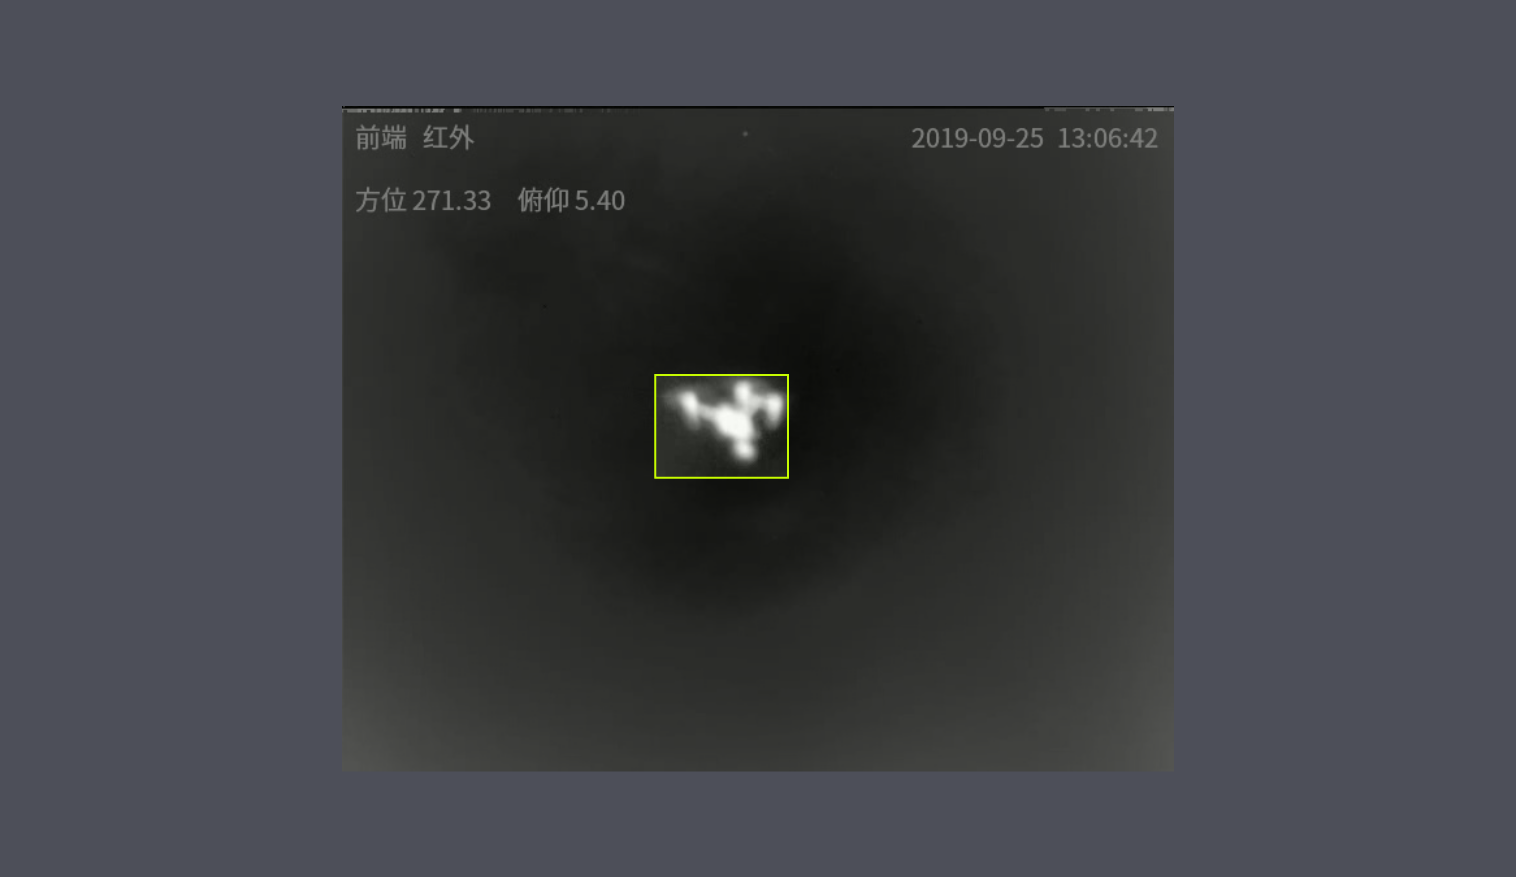
\includegraphics[width=0.4\textwidth]{1.png}}}
    \hspace{2em}
    \subfigure{\label{dataset12}}\addtocounter{subfigure}{-2}
    \subfigure{\subfigure[正常目标示例~2]{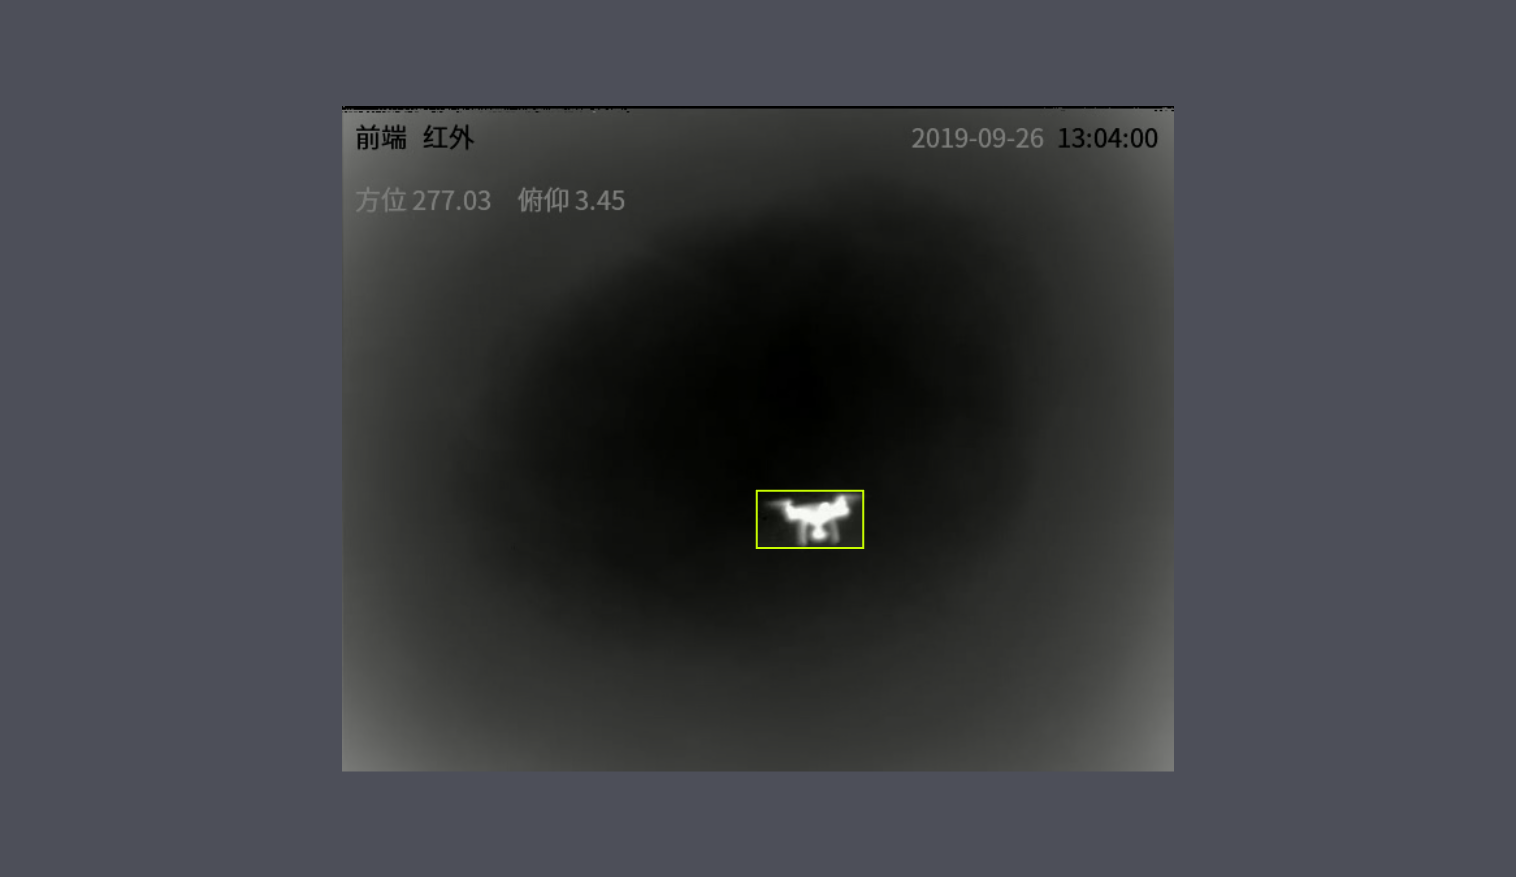
\includegraphics[width=0.4\textwidth]{2.png}}}
    \end{minipage}

    \centering
    \begin{minipage}{\textwidth}
    \centering
    \subfigure{\label{dataset21}}\addtocounter{subfigure}{-2}
    \subfigure{\subfigure[小目标示例~1]{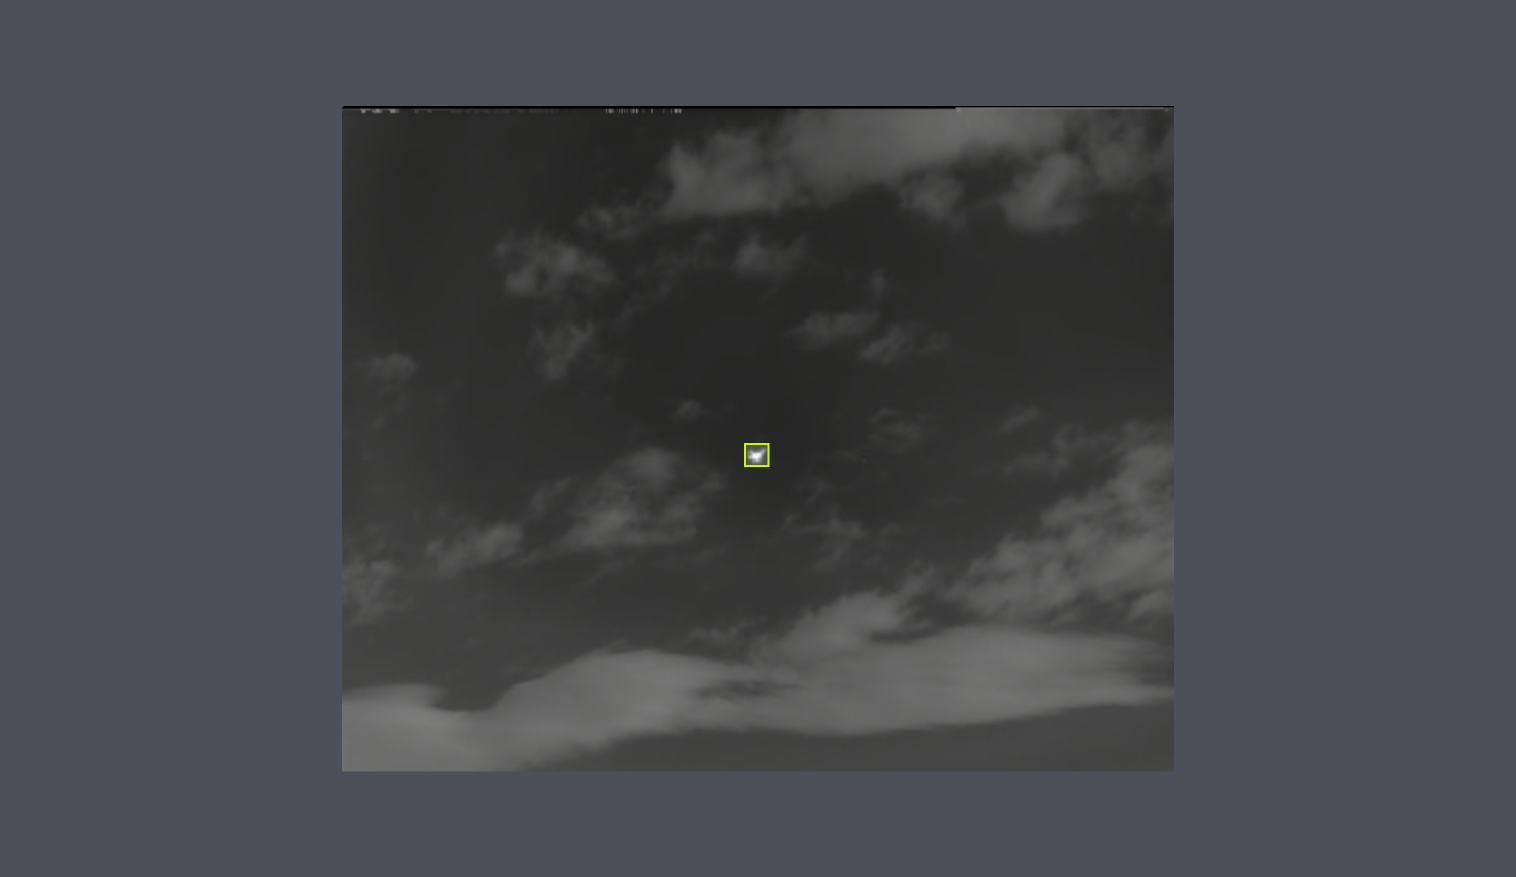
\includegraphics[width=0.4\textwidth]{5.png}}}
    \hspace{2em}
    \subfigure{\label{dataset22}}\addtocounter{subfigure}{-2}
    \subfigure{\subfigure[小目标示例~2]{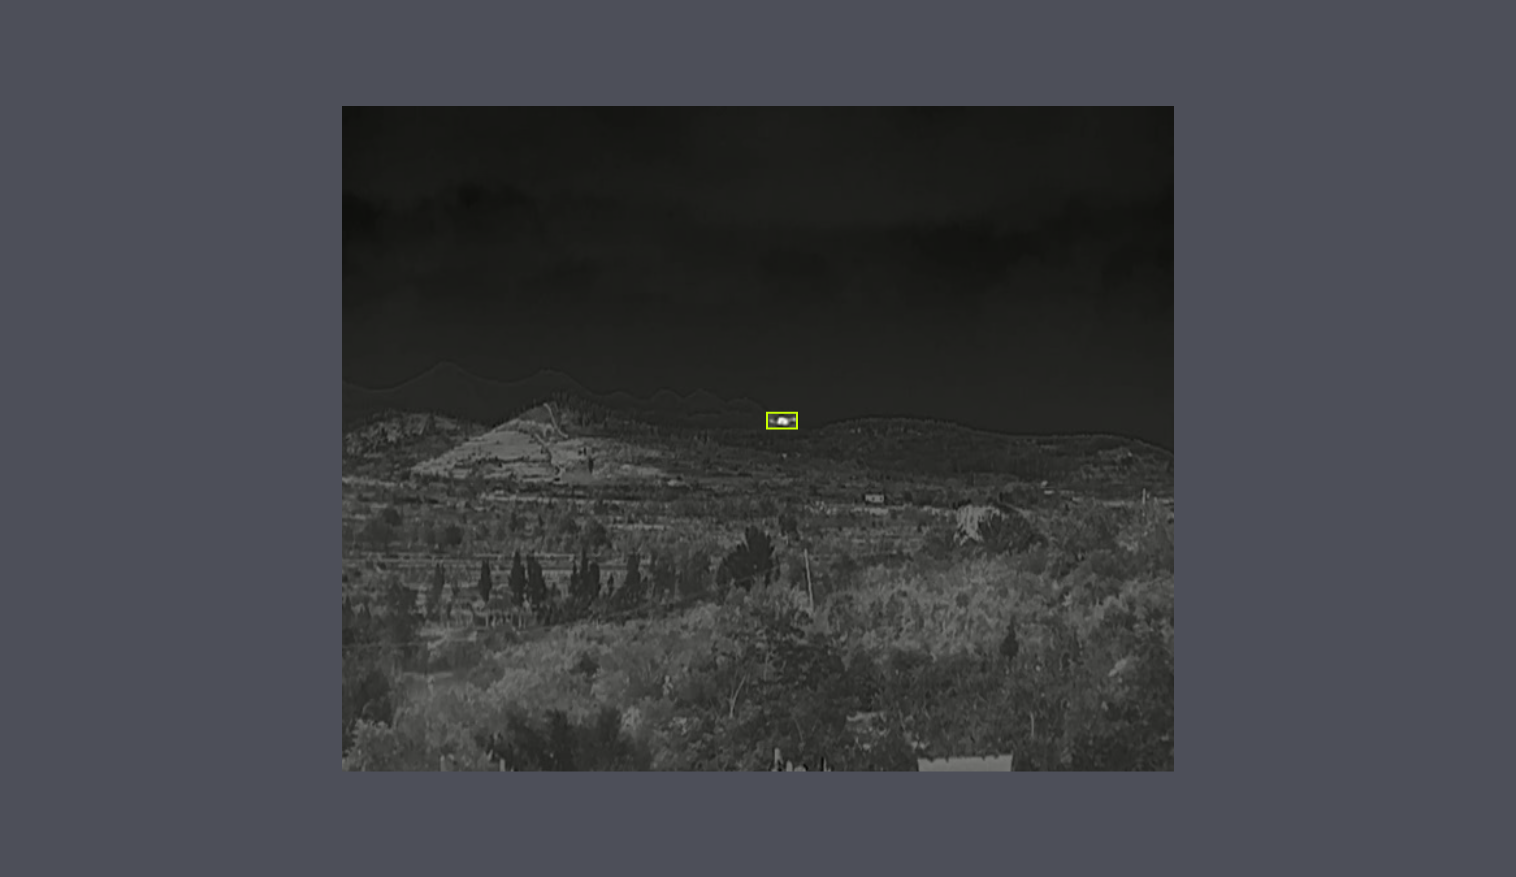
\includegraphics[width=0.4\textwidth]{6.png}}}
    \end{minipage}

    \centering
    \begin{minipage}{\textwidth}
    \centering
    \subfigure{\label{dataset31}}\addtocounter{subfigure}{-2}
    \subfigure{\subfigure[遮挡目标示例~1]{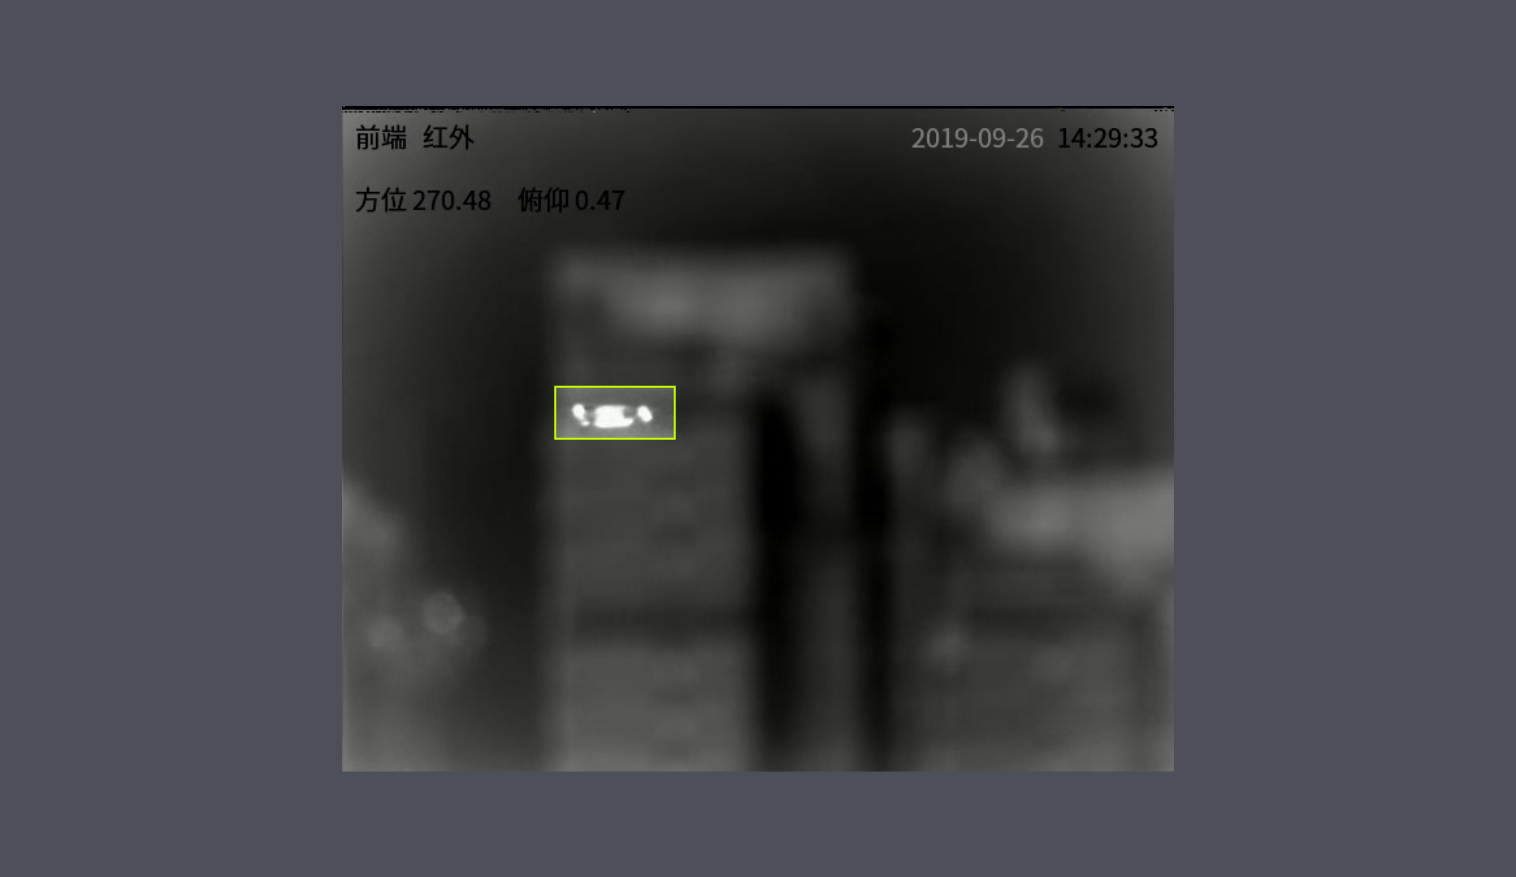
\includegraphics[width=0.4\textwidth]{3.png}}}
    \hspace{2em}
    \subfigure{\label{dataset32}}\addtocounter{subfigure}{-2}
    \subfigure{\subfigure[遮挡目标示例~2]{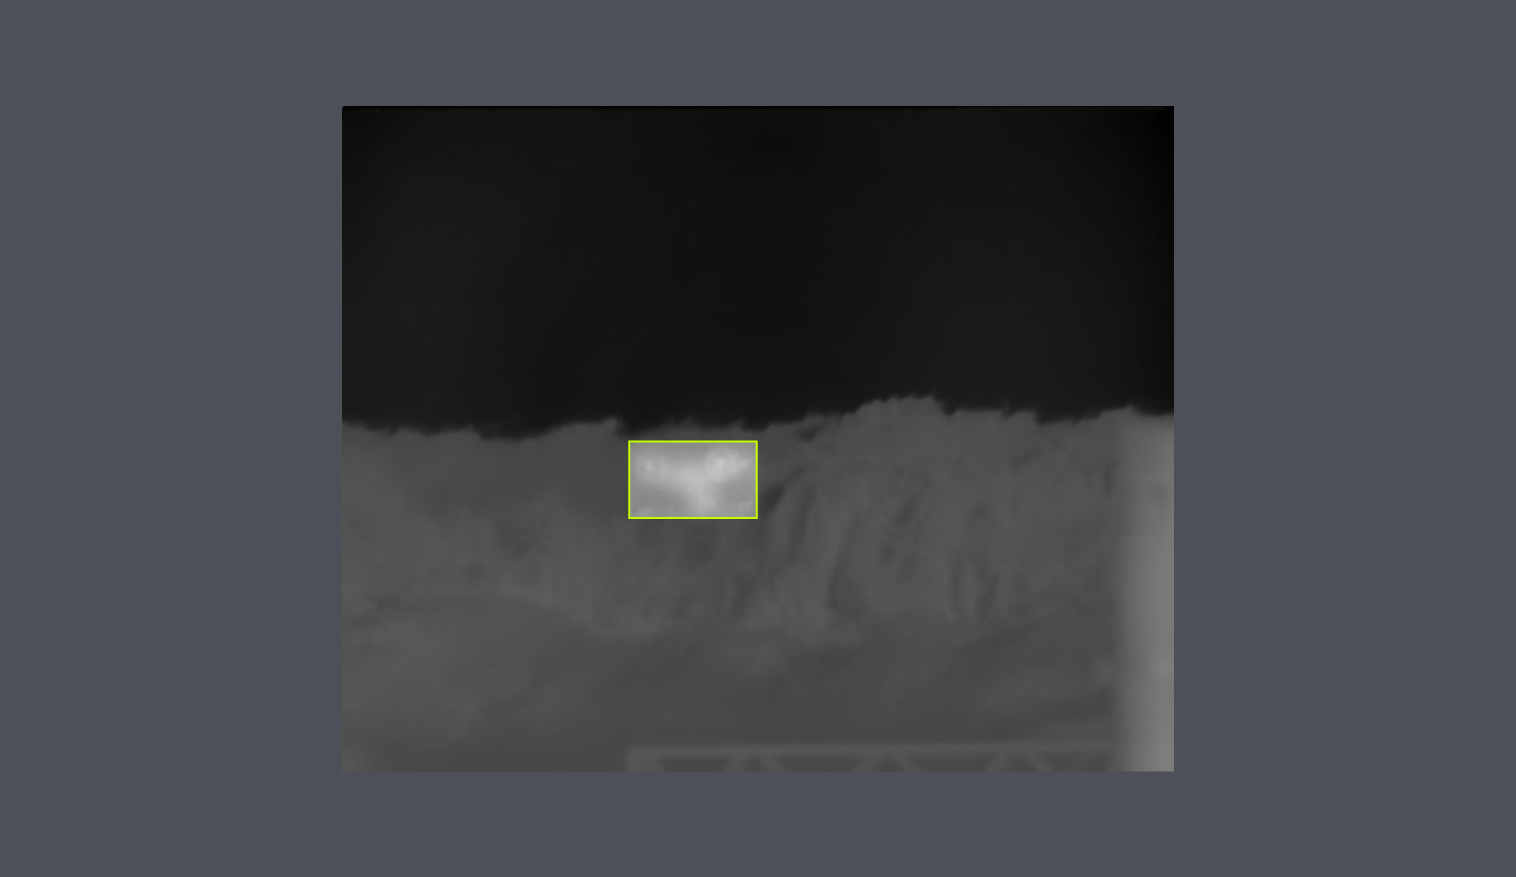
\includegraphics[width=0.4\textwidth]{4.png}}}
    \end{minipage}

    \vspace{0.2em}
    \caption{数据集图像示例}
    {\label{dataset}}
\end{figure}


\section{深度学习网络模型基本算法YOLOv5}
本课题算法的主干网络模型采用YOLOv5网络,网络的结构如图\ref{yolo1}所示,
该模型按照推理流程顺序主要可以分成
输入端、Backbone、Neck、Prediction这四个部分。

\begin{figure}[h]
    \centering
    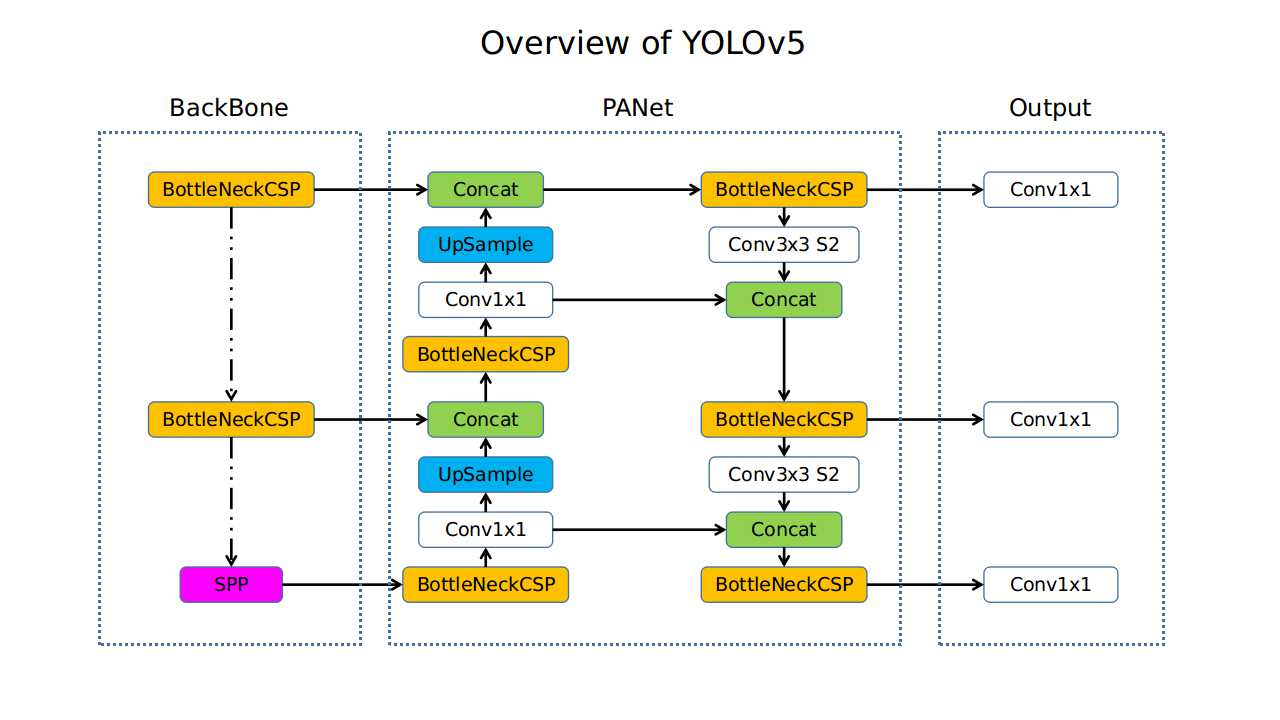
\includegraphics[width = 0.8\textwidth]{yolov5结构.jpg}
    \caption{yolov5网络结构}
    \label{yolo1}
\end{figure}

\subsection{输入端}
YOLOv5网络的输入端就是输入图像的模块,
既可以向网络提供原始的图像输入,
也可以在这个部分对图像进行预处理
和数据增强,
此外还能进行算法的准备工作,比如锚框的
自适应计算等。

\subsection{Backbone}
Backbone的主要作用是初步提取特征图。其中典型的模块是Focus模块、CBL模块以及CSP模块。

\subsubsection{Focus模块}
Focus模块是主要功能是对输入图像进行初步处理,将图像进行切分,以类似降采样的间隔取值方式将原图像中的像素点拆分后组合为新的小图像,这样处理的作用是扩充了输入的通道数,同时没有信息丢失的问题。对于具体的某张输入图像,如果应用$4\times4$规格的Focus切片处理,就可以将输出通道由原本的BGR形式的3个通道扩充到12个通道,每张输出特征图尺寸则会变成输入图像的$\frac{1}{4}$。最后对切分后的图片应用卷积运算。Focus切片处理的过程如图\ref{focus}所示。

\begin{figure}[h]
  \centering
  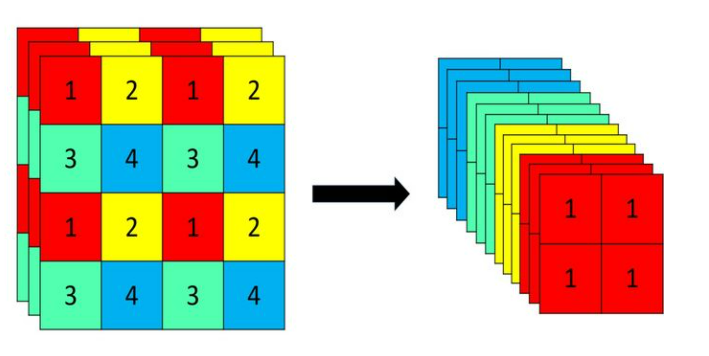
\includegraphics[width = 0.8\textwidth]{focus.png}
  \caption{Focus切片示意图}
  \label{focus}
\end{figure}

\subsubsection{CBL模块}
CBL模块是卷积神经网络的基本组成模式,
结构如图\ref{cbl}所示,
由卷积、归一化、激活函数三个部分组成。
CBL的主要作用是通过卷积采集特征。
其中的激活函数默认是Leaky ReLU,Leaky Rectified Linear Unit是一种基于 ReLU 的激活函数,但它对于负值的斜率很小,而不是平缓的斜率。 斜率系数是在训练之前确定的,即它不是在训练期间学习的。 这种类型的激活函数在我们可能遭受稀疏梯度的任务中很受欢迎。

\begin{figure}[h]
  \centering
  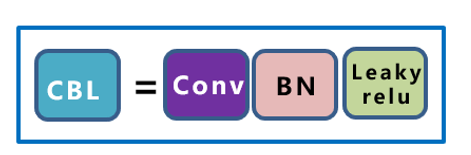
\includegraphics[width = 0.5\textwidth]{CBL.png}
  \caption{CBL模块组成示意图}
  \label{cbl}
\end{figure}

\begin{figure}[h]
  \centering
  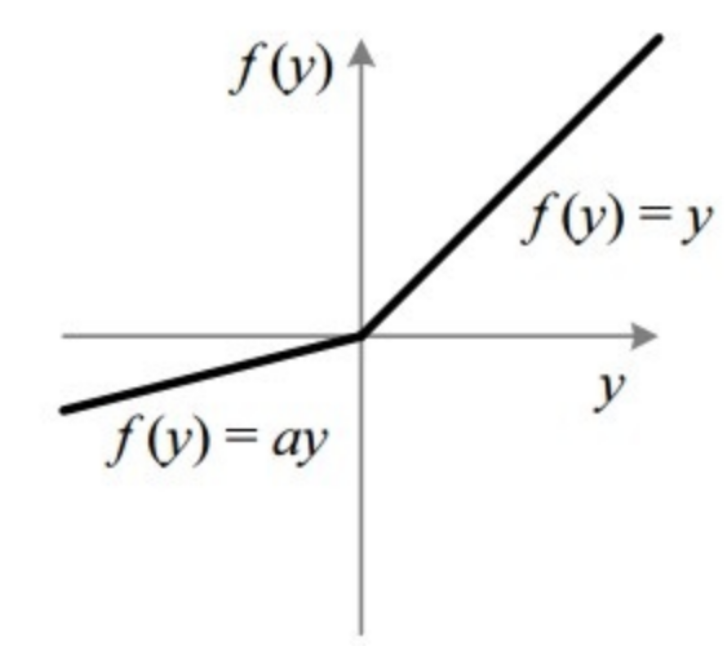
\includegraphics[width = 0.4\textwidth]{leakyrelu.png}
  \caption{Leaky ReLU示意图}
  \label{relu}
\end{figure}

\subsubsection{CSP模块}
CSP模块的主要作用是解决以往的网络推理计算中计算量过大的问题,具体地处理思路是,通过缓解网络计算优化中的过多重复梯度信息的现象来降低网络中过高的计算负载。CSP 模块把输入特征图分割为两部分,并且在后续处理中通过合并的方式兼顾梯度的充分组合和计算量的优化。
YOLOv5网络的Backbone部分采用创新的CSPDarknet,达到提取输入图像的重要特征的目的。CSPDarknet的主要优势在于简化了梯度信息的传递,同时减少了整个YOLOv5算法系统的参数量和计算量。

\begin{figure}[h]
  \centering
  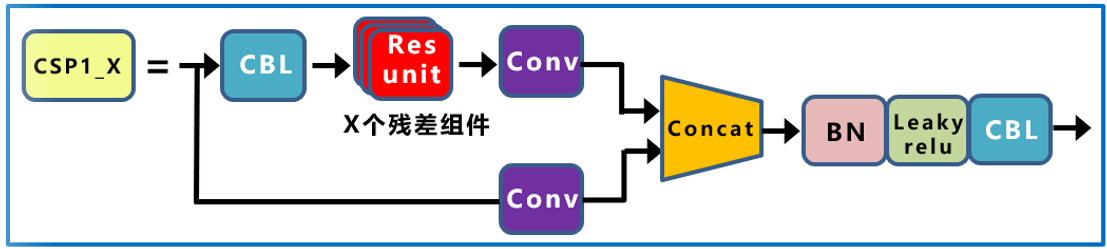
\includegraphics[width = 0.8\textwidth]{CSP.png}
  \caption{CSP模块组成示意图}
  \label{csp}
\end{figure}

\subsection{Neck及Prediction}
Neck部分主要由FPN和PAN组成。FPN指的是特征金字塔网络(Feature Pyramid Network),特征金字塔是一种
用于检测不同尺度物体的系统。该算法模块利用固有的多尺度,
深度卷积网络的金字塔层次结构以边际额外成本构建特征金字塔。研究人员开发了具有横向连接的自上而下的架构,
主要作用是建立各个尺度的语义特征图。这种架构作为通用特征提取器在不同场景均显示出出色的性能。
FPN对小尺度目标检测效果更好。FPN可以利用经过top-down模型后的那些上下文信息(高层语义信息)。
对于小目标而言,FPN增加了特征映射的分辨率(即在更大的feature map上面进行操作,这样可以获得更多关于小目标的有用信息)。

PANet是一种旨在提升信息的路径聚合网络结构(Path Aggregation Network)。
具体来说,PANet增强了整个特征层次结构中
自下而上的低层精确定位信号,提出了自适应特征池,
它将特征网格和所有特征级别联系起来,进而在每个特征级别中生成有用的信息
直接传播到以下提议子网,缩短了较低层和最顶层特征之间的信息路径。
PANet在实例分割和目标检测等任务中均有着优秀的性能表现。

Prediction部分包含上级输出的特征向量,并通过输入的特征向量得出坐标值、置信度,结合损失函数和后处理函数得出检测结果。

\subsection{YOLOv5基础网络性能验证与分析}
本节将在自建数据集上对YOLOv5基础网络的性能进行验证,将其与常见算法SSD和Faster R-CNN进行对比,并分析YOLOv5算法的优势。
为了证明基础YOLOv5算法在红外无人机目标检测任务中的有效性,本节将其与目标检测算法SSD以及Faster R-CNN进行对比实验。
本章提到的YOLOv5基础算法用深度学习网络框架Pytorch进行实现、训练和测试。操作系统为Windows 10,使用的主要软件为python。实验平台采用的CPU型号为Intel Core i7-11700k,GPU型号为NVIDIA GeForce RTX 3080Ti,显存容量为12GB。训练过程中使用GPU进行加速。



\begin{table}[htbp]
  \caption{不同算法对红外无人机数据集的检测结果}
  \vspace{0.5em}\centering\wuhao
  \begin{tabular}{ccc}
  \toprule
  检测算法 & mAP & 推理时间(ms)\\
  \midrule
  Faster R-CNN & 0.625 & 12.5\\
  SSD & 0.705 & 10.3\\
  YOLOv3 & 0.904 & 7.5\\
  YOLOv5 & 0.919 & 2.5\\
  \bottomrule
  \end{tabular}
  \label{t11}
\end{table}

根据表\ref{t11}中的实验结果,Faster R-CNN在本文自建红外图像无人机目标检测数据集的mAP较低,同时会消耗更多的推理时间。这是因为Faster R-CNN算法虽然相对于R-CNN算法有所改进,但是仍然采用二阶段检测方式,先进行提名候选框后进行目标检测,这种检测方式虽然一定程度上保证了检测精度,但是会使得算法总体的检测耗时较长。而SSD算法在单阶段检测的同时,引入了特征金字塔结构,充分利用了多尺度目标的特征,因而能在检测精度和推理时间上都有较好的表现。而YOLOv3由于经过了几次迭代和改进,所以精度上比SSD算法和Faster R-CNN算法更高且检测速度较快。由于YOLO系列算法直接采用了单阶段检测,较大程度地减少了推理时间。但是由于网络结构中没有充分利用多尺度特征信息,因此在尺度变化较大的数据集上精度不高。而YOLOv5网络在YOLOv3的基础上,应用了很多提升精度的改进,如增加了PANet、改进了损失函数等,也应用了很多提升速度的改进,如应用了CSP模块等,因此在实验结果中体现出YOLOv5的检测精度和推理时间都是最优的,因此本文选择YOLOv5算法作为红外无人机目标检测算法的基础。

\section{数据增强算法}
由于深度学习算法通常需要大量的数据进行学习,因此在原始数据集的基础上,将基础网络结合数据增强算法能在一定程度上提升算法的性能。因此本节将对常见的图像增强算法进行实验,在实验结果的基础上针对红外图像目标检测任务提出一种图像填充算法,此外还将针对红外无人机目标检测任务中的背景较为复杂的特性提出一种图像拼接的数据增强算法。

\subsection{主流的图像增强算法}
目前计算机视觉领域常见的图像增强处理算法可以根据对输入图像的处理方式划分为
空域增强算法和频域增强算法。空域指的是图像的像素维度,即对组成原始图像的各个像素直接处理,常见的空域增强方法有降噪、直方图均衡等。
频域指的是图像的频率域,一般包含图像的变化快慢信息。因此频率域的增强往往关注图像的边缘等从频率角度观察会表现得更为直观的信息。
考虑到处理的复杂度和时间成本,本文从空域角度重点研究图像的增强算法。

对输入图像进行空域增强的过程可以定义成如式\ref{aug1}所示:

\begin{equation}
  g(x, y)=T[f(x, y)]
  \label{aug1}
\end{equation}

式中$f(x, y)$代表输入的原始图像,$T$是一种空间域变换的定义,$g(x, y)$表示经过空域增强算法处理后的输出图像。

\subsubsection{Inversion}
由于主流的目标检测算法应用的场景都是基于BGR图像的,不适于检测红外目标,因此需要将红外图像进行预处理以达到使红外图像更接近BGR图像的目的,通过域迁移的思想使得网络能够更加适应处理后的红外图像。一般用于目标检测所用的RGB图像都是白天所摄,通常情况是背景较亮,目标较暗。但是红外图像成像为辐射特性,故一般背景辐射较弱而目标辐射较强。因此,考虑采用Inversion操作对输入的原始图像进行处理,Inversion处理的过程如式\ref{inv1}所示:
\begin{equation}
  f: x_{p}=u-x
  \label{inv1}
\end{equation}

式中,$x_{p}$表示Inversion处理后的输出图像,$u$表示图像系统中像素强度值的上限,特别地,对于8bit色深的图像色彩系统,$u$的值为255。$x$表示输入的原始图像。

\subsubsection{直方图均衡}
通常情况下,红外图像的灰度往往集中在某个值域内,这是因为红外成像系统采集到的图像对比度较低,因此需要运用直方图均衡的算法将输入图像的灰度均匀地分散到更大的范围内,使得图像的整体对比度提升,从而降低后续的目标检测算法的处理难度。
一般情况下,直方图均衡处理算法的过程如下: 

(1)对输入图像,统计其每个像素点的灰度值分布情况,计算方法如式\ref{he1}所示。
\begin{equation}
  \mathrm{p}_{r}\left(r_{k}\right)=\frac{n_{k}}{n} \quad k=0,1,2, \ldots, L-1
  \label{he1}
\end{equation}

其中$n$代表输入图像的像素点总个数,$n_{k}$代表灰度经离散化处理后处于$r_{k}$间隔的像素点个数。

(2)对图像的灰度分布情况,可以得到变换后的图像灰度分布,计算过程如式\label{pix trans}所示:
\begin{equation}
  \mathrm{s}_{k}=T\left(r_{k}\right)=\sum_{j=0}^{k} p_{r}\left(r_{j}\right)=\sum_{j=0}^{k} \frac{n_{j}}{n} \quad k=0,1,2, \ldots L-1
  \label{pix trans}
\end{equation}

通过式\ref{pix trans}
可以获得处理之后像素点的灰度分布情况,其中$r_{k}$表示处理前的像素点灰度值,$s_{k}$表示处理后输出的像素点的灰度值。

直方图均衡是一种常见的提高输入图像对比度的方式,同时还具有计算时间负载较小的优势,但是该算法存在的问题是可能造成图像中细粒度特征的强度降低,针对这个问题后续的研究人员提出了对比度受限的直方图均衡等方法。

\subsubsection{USM锐化}
对于大多数情况下的目标检测任务,目标相对背景都是有较明显的轮廓,因此可以采用锐化处理方法进一步加强物体的边界,进而增强检测效果。

锐化的本质是对原图像实现高通滤波,得到原图像的高频分量,也就是对原图像中的边缘部分进行了增强。计算机视觉图像增强算法中一种性能较好的锐化方法是USM(Unsharp Mask)算法,这种处理方法的主要思想是先获得输入图像中变化较慢的低频分量,之后利用该低通分量对原始图像进行掩模处理,意图是使原始图像消去自身的低频分量后保留高频分量,从而达到锐化图像的目的。
基于USM的锐化算法比直接使用利用算子对输入图像进行卷积的锐化方式应用更加广泛,原因是USM算法一定程度上不会受到较弱的干扰噪声的影响。
\begin{equation}
  I_{sharpend}=I_{original}+(I_{original}-I_{blurred})*a
\end{equation}

式中$I_{sharpend}$表示锐化后的图像,$I_{original}$表示原始图像,$I_{blurred}$表示模糊后的原始图像,$a$表示权重系数。

\subsection{通道填充算法}
本章结合第2章中分析的红外图像的成像特点,认为红外图像存在信息量不足等特点,使得在可见光目标检测领域性能优秀的目标检测算法难以直接通过迁移就取得良好的性能。因此本节中提出了一种基于通道填充的红外图像数据增强算法,核心思想是抓住红外图像和可见光图像之间的主要差异,即红外图像仅有1个灰度通道进行信息的表达,而可见光图像通常包含BGR3个通道,考虑将原始的红外图像由单通道填充为和可见光图像相同的3个通道,增加参与训练的数据量,提高YOLOv5目标检测算法模型的学习效果和检测性能。
通道填充算
法的流程如图\ref{tdtc}所示。

\begin{figure}[h]
  \centering
  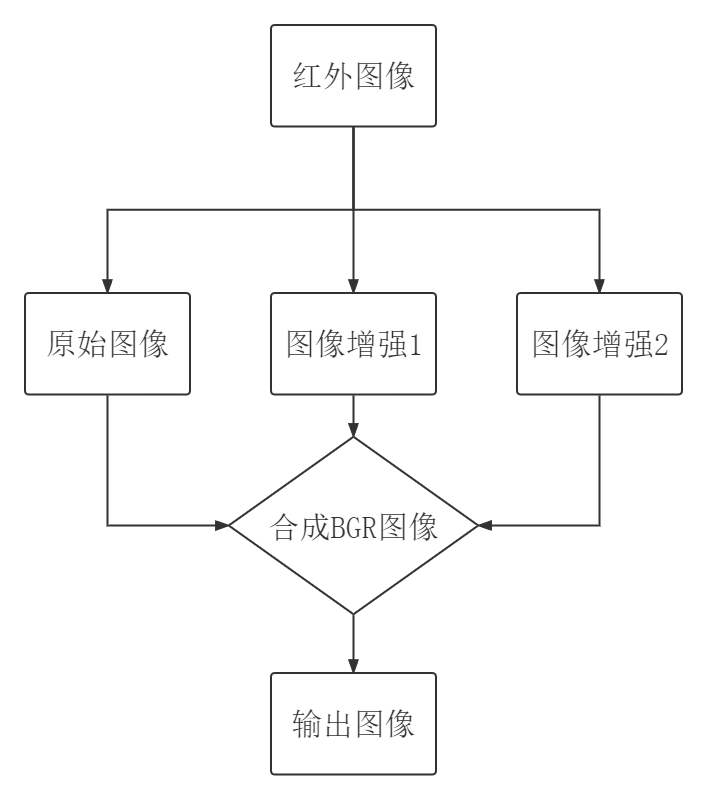
\includegraphics[width = 0.6\textwidth]{通道填充流程图.png}
  \caption{通道填充算法流程图}
  \label{tdtc}
\end{figure}

由于该算法输出的图像包含3个通道,其中1个是原始的红外灰度图像,另外两个通道采用以下3种图像增强算法中的两个,具体选择策略经过实验对比后确定。

(1)Inversion。主要目的在于增强图像的信息多样性,同时使得红外图像更加贴近可见光图像的特性。

(2)CLAHE。主要作用是提升输入红外图像的对比度,和普通HE算法的主要区别是CLAHE算法对整个图像进行分区后再进行HE处理,能更细粒度地起到增强图像对比度的作用。

(3)USM变换。主要目的在于抑制噪声的同时进行图像的锐化,强化目标的边缘。本文使用高斯模糊后的USM变换进行锐化。

\begin{figure}[htbp]
	\centering
	\begin{minipage}{0.49\linewidth}
		\centering
		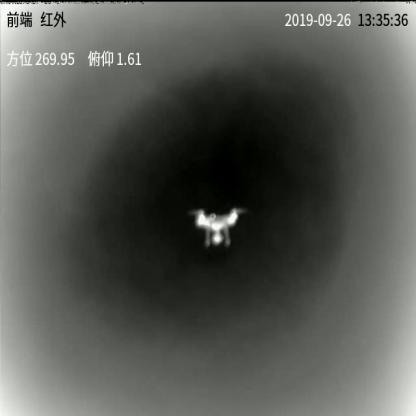
\includegraphics[width=0.9\linewidth]{原图1.JPG}
		\caption{原图示例}
		\label{txzq11}%文中引用该图片代号
	\end{minipage}
	\begin{minipage}{0.49\linewidth}
		\centering
		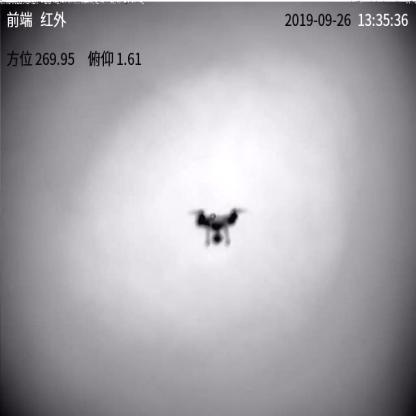
\includegraphics[width=0.9\linewidth]{inv1.JPG}
		\caption{Inversion处理示例}
		\label{txzq21}%文中引用该图片代号
	\end{minipage}
	%\qquad
	%让图片换行,
	
	\begin{minipage}{0.49\linewidth}
		\centering
		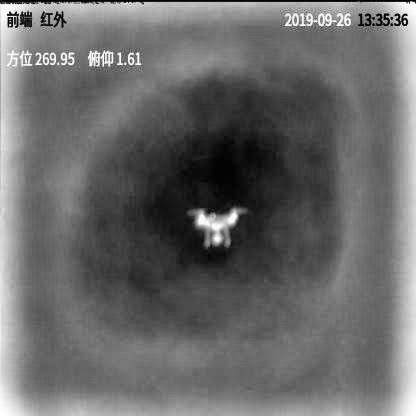
\includegraphics[width=0.9\linewidth]{clahe1.JPG}
		\caption{CLAHE处理示例}
		\label{txzq31}%文中引用该图片代号
	\end{minipage}
	\begin{minipage}{0.49\linewidth}
		\centering
		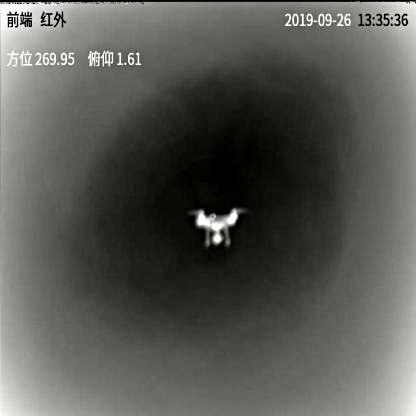
\includegraphics[width=0.9\linewidth]{usm1.JPG}
		\caption{USM处理示例}
		\label{txzq41}%文中引用该图片代号
	\end{minipage}
  \label{txzq}
\end{figure}

增强后的图片效果如图\ref{txzq11}、\ref{txzq21}、\ref{txzq31}、\ref{txzq41}所示,其中\ref{txzq11}表示原图像,\ref{txzq21}表示原图经过Inversion处理后的图像,\ref{txzq31}表示原图像经过CLAHE处理后的图像,\ref{txzq41}表示原图像经过USM处理后的图像。

\subsection{图像拼接算法}
由于在红外无人机目标检测的场景下,无人机目标往往可能从探测器的各方向出现,目标的背景变化较多,因此考虑采用一种图像拼接的数据增强算法,将训练数据中的目标数增多,同时丰富训练数据图像中的背景,增强模型的泛化能力,从而增强网络对目标的检测能力。

该算法的实现方法是,从训练集中随机抽取4个图像,将这4张图像进行拼接后生成一张与原始图像相同大小的新图像输入网络。

\begin{figure}[htbp]
	\centering
	\begin{minipage}{0.49\linewidth}
		\centering
		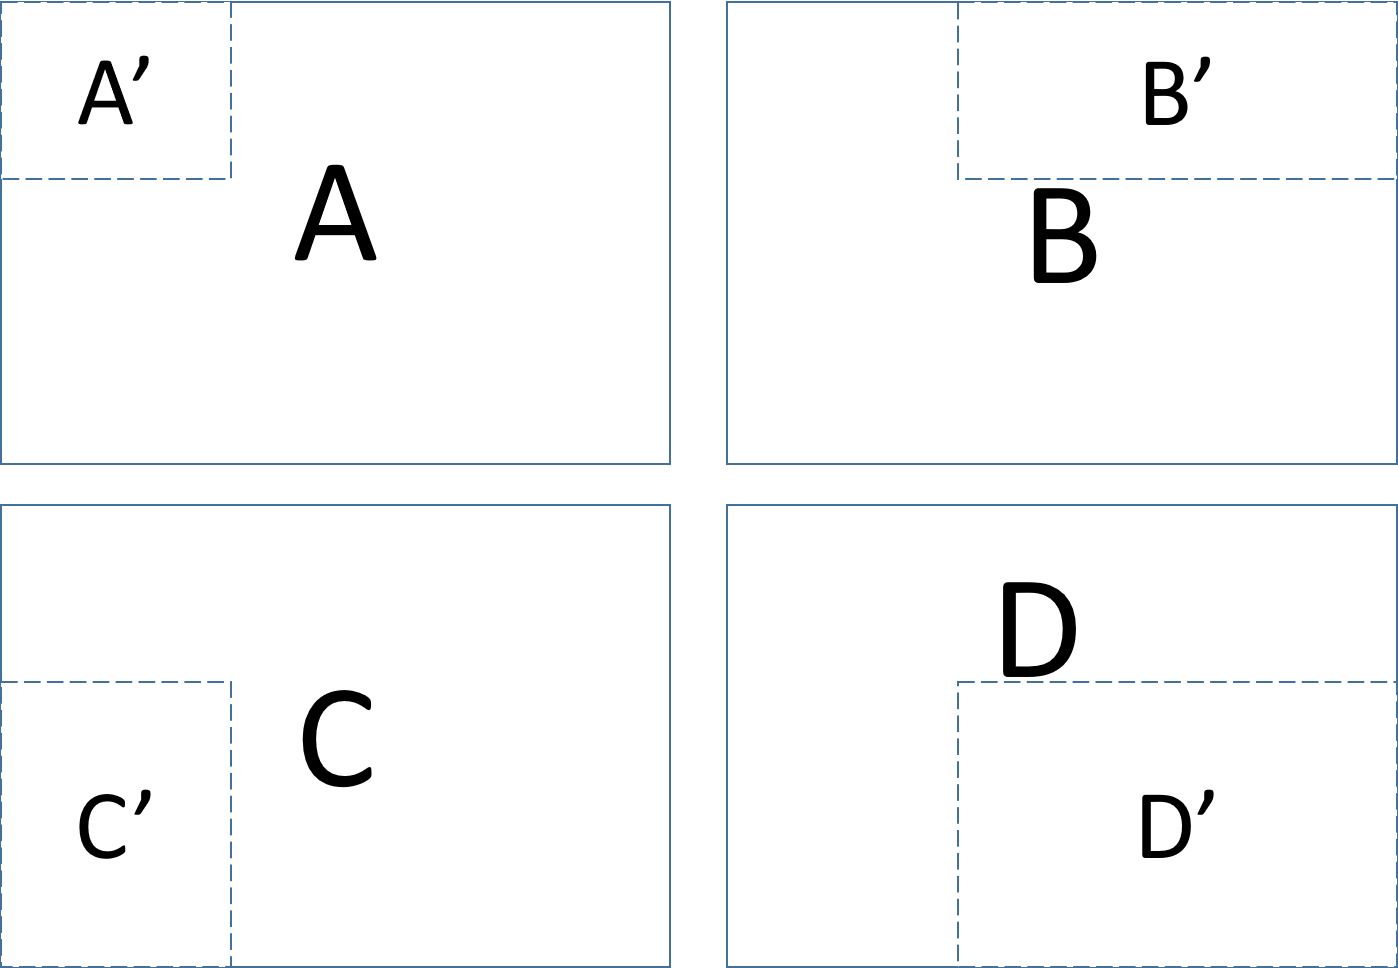
\includegraphics[width=0.9\linewidth]{txpj1.PNG}
		\caption{原始图像及切割示意图}
		\label{txpj1}%文中引用该图片代号
	\end{minipage}
	%\qquad
	\begin{minipage}{0.49\linewidth}
		\centering
		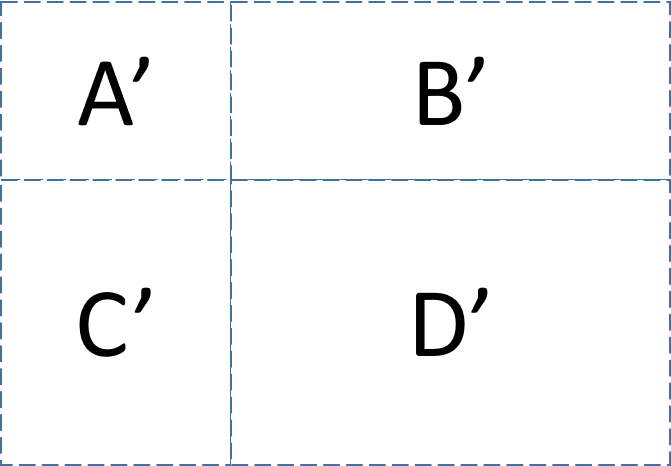
\includegraphics[width=0.9\linewidth]{txpj2.PNG}
		\caption{拼接结果图}
		\label{txpj2}%文中引用该图片代号
	\end{minipage}
\end{figure}

如图\ref{txpj1}所示,图像拼接算法的实现流程是:

(1)图中A、B、C、D分别是4张大小尺寸相同的原始图像,假设长为$w$,宽为$h$。

(2)在图像矩形的中心区域范围内随机生成一个坐标作为四张图片的切割点(例如生成点坐标为$(x,y)$,则限制其中$x\in[0.4w,0.7w],y\in[0.4h,0.7h]$)。

(3)将每张图片分割成四个矩形后,取每张图片的不同部分,即在图A中取A'(原图A的左上部分),在图B中取B'(原图B的右上部分),在图C中取C'(原图C的左下部分),在图D中取D'(原图D的右下部分)。

(4)将4张小图按其在原图中的位置放置后得到结果图,如图\ref{txpj2}所示。

如图\ref{txpj}所示,对随机4张红外无人机数据图像应用图像拼接算法后得到一张包含更丰富背景、更多标注目标的训练样本图。

\begin{figure}[htpb]
  \centering
  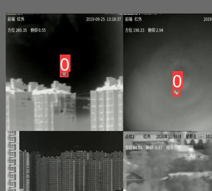
\includegraphics[width = 0.5\textwidth]{图像拼接1.png}
  \caption{图像拼接效果图}
  \label{txpj}
\end{figure}

\section{改进损失函数}
YOLOv5网络的损失函数主要由三部分组成:第一部分是bounding box损失,主要根据预测目标框和真值目标框的重合程度进行计算。第二部分是置信度损失,第三部分是分类误差。

其中对于bounding box的损失函数主要是基于$IoU$(交并比,Intersection over Union)进行计算。$IoU$一般表示预测框与真值框面积的交并比,即二者相交的面积除以二者所占的总面积。
\begin{equation}
  I o U=\frac{|A \cap B|}{|A \cup B|}
\end{equation}

这样一种计算方式相对于之前的基于点到点之间距离的MSE损失函数已经有较大的优势,主要体现在:

(1)MSE损失函数由于是按点距离计算,因此对于任务目标的尺寸变化较为敏感,尺寸变化往往会引起损失函数的无意义波动。

(2)MSE损失函数从点距离出发,忽略了目标框各点之间的关联。因此基于$IoU$的损失函数已经在一定程度上反映了预测框与真值框之间的误差关系。

而$IoU$损失函数有两个重要特性,使得它能作为很多计算机视觉算法的损失函数。

(1)$\mathcal{L}=1-IoU$满足非负性、同一性、对称性、三角不等性等所有损失函数的特性。

(2)$IoU$相对于问题的规模是不变的。这意味着两个任意形状之间的相似性独立于它们的空间规模。

然而基于$IoU$的损失函数也存在一定的问题。

(1)当预测框与真值框没有相交区域时,$IoU$值为0,此时损失loss为0,无法进行梯度回传,也就是无法进行模型训练。

(2)$IoU$还是无法精确地衡量预测框与真值框之间的误差情况,尤其是在$IoU$为0时,预测框与真实框之间的距离变得无法量化。

因此,针对$IoU$的这一问题,为了增强算法对红外无人机目标检测任务中的目标框定位能力,可以引入一种更加完善的$GIoU$损失函数。设$I o U=\frac{\mathcal{I}}{\mathcal{U}}$
,其中$\mathcal{I}$表示预测框与真值框相交部分面积,$\mathcal{U}$表示预测框与真值框合并部分面积,则$GIoU$的计算公式是:
\begin{equation}
  G I o U=I o U-\frac{A^{c}-\mathcal{U}}{A^{c}}
\end{equation}

其中$A^{c}$表示预测框和真值框的最小闭包区域的面积。

\begin{figure}[htbp]
  \centering
  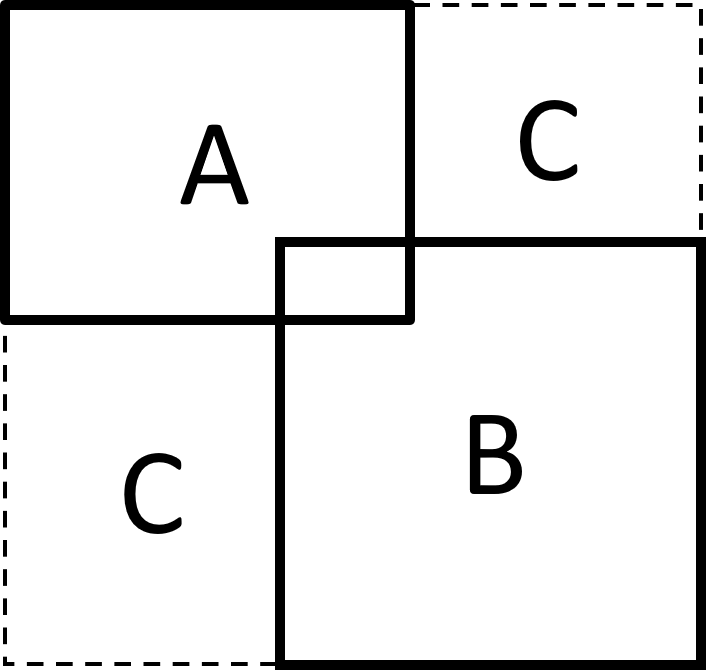
\includegraphics[width = 0.5\textwidth]{giou示意.png}
  \caption{GIoU示意图}
  \label{gi}
\end{figure}

如图\ref{gi}所示,$GIoU$的计算流程是:

(1)找到预测框(图\ref{gi}中区域A)和真值框(图\ref{gi}中区域B)的边界点,计算闭包区域(图\ref{gi}中整个虚线包围的矩形区域)面积。

(2)计算预测框和真值框相交部分和合并部分面积,求得补集部分(图\ref{gi}中区域C)面积。

(3)代入公式$G I o U=I o U-\frac{A^{c}-\mathcal{U}}{A^{c}}$以及$\mathcal{L}_{G I o U}=1-G I o U$得到$\mathcal{L}_{G I o U}$。

$GIoU$是经过改进的$IoU$计算方法,有如下几个特点:

(1)与$IoU$相似,也是一种距离度量,作为损失函数满足损失函数的需求。

(2)$GIoU$除了关注重叠区域不同,还关注了非重叠区域,能够更好的反应重合度。

(3)$GIoU$对目标的尺度不敏感。

(4)当预测框与真值框重合时,$GIoU=IoU$,即$GIoU$的上限是$IoU$,因此训练时不会出现梯度爆炸的情况。

\section{实验结果与分析}
本节将在YOLOv5网络的基础上,应用本章提出的数据增强算法以及损失函数的改进方案,在红外图像无人机目标数据集上进行性能测试和对比,并对实验结果进行分析。


\subsection{实验环境与参数}
本章提到的算法用深度学习网络框架Pytorch进行实现、训练和测试。操作系统为Windows 10,使用的主要软件为python。实验平台采用的CPU型号为Intel Core i7-11700k,GPU型号为NVIDIA GeForce RTX 3080Ti,显存容量为12GB。训练过程中使用GPU进行加速。

\subsection{不同算法对比与分析}
在上述环境下,进行算法的训练和测试,以mAP和推理时间作为评价指标,对比结果列在表\ref{m1}中。

\begin{table}[htbp]
  \caption{不同算法对红外无人机数据集的检测结果}
  \vspace{0.5em}\centering\wuhao
  \begin{tabular}{cc}
  \toprule
  检测算法 & mAP\\
  \midrule
  YOLOv5 & 0.919\\
  Ours(YOLOv5+Inversion数据增强) & 0.924\\
  Ours(YOLOv5+CLAHE数据增强) & 0.918\\
  Ours(YOLOv5+USM数据增强) & 0.913\\
  Ours(YOLOv5+Inversion+CLAHE通道填充) & 0.930\\
  Ours(YOLOv5+Inversion+USM通道填充) & 0.913\\
  Ours(YOLOv5+CLAHE+USM通道填充) & 0.910\\
  Ours(YOLOv5+Inversion+CLAHE通道填充+图像拼接) & 0.929\\
  Ours(YOLOv5+Inversion+CLAHE通道填充+GIoU) & 0.932\\
  Ours(YOLOv5+Inversion+CLAHE通道填充+图像拼接+GIoU) & 0.937\\
  \bottomrule
  \end{tabular}
  \label{m1}
\end{table}

由表\ref{m1}中所示数据可以看出,YOLOv5目标检测算法在本文的检测任务中已经能取得较好的精度。本节首先对基础的数据增强方法进行了对比实验(即对训练数据采用Inversion变换、CLAHE变换、USM变换其中之一处理后生成训练数据)。实验结果显示,在进行Inversion数据增强后,YOLOv5算法的检测精度得到了小幅度的提升,这是由于部分图像在经过Inversion后和原始图像相差较大,使得网络学习到了更为丰富的特征。而应用CLAHE数据增强方法后算法的检测精度基本不变,应用USM数据增强方法后算法的检测精度略有下降,这是因为USM虽然在一定程度上抑制噪声,但是由于有些图像本身的信噪比不高,有相当数量的图像经过USM后增强了噪声,影响了模型的训练效果。随后本节对本文提出的通道填充算法进行了对比实验。实验结果显示,YOLOv5+Inversion+CLAHE通道填充取得了相比于单纯应用Inversion数据增强后的YOLOv5网络取得了更高的检测精度,这是因为网络在经过不同的三通道数据进行训练后增强了特征提取的能力。在应用了图像拼接算法后,算法的精度并没有提高,虽然理论上模型对复杂背景的检测能力得到增强,但是本文采用的训练集已经包含了大量的复杂背景样本,因此单纯应用图像拼接后会使得背景的干扰强度过大,可能一定程度上降低了模型的泛化能力。而后本节对应用了GIoU损失函数的网络结构进行了对比实验,结果显示YOLOv5+Inversion+CLAHE通道填充+图像拼接+GIoU的红外无人机目标检测算法取得了比其他算法更高的检测精度,这一方面是因为GIoU损失函数的改进提高了网络对于目标预测框的定位能力,另一方面是因为图像拼接后,目标框和预测框更容易出现更大的偏差,原始的IoU损失函数性能下降,因此图像拼接算法在配合GIoU损失函数后表现出了更高的检测精度。

\section{本章小结}
本章首先介绍了本文采用的自建红外无人机目标数据集的制作过程。之后本章介绍了本文采用的目标检测算法基于的YOLOv5神经网络的结构,并且在数据集上进行了对比实验,证明了在红外无人机目标检测任务中,YOLOv5算法的检测能力强于常见的YOLOv3算法、Faster-RCNN算法以及SSD算法。此后本章分析了本课题主要面临的问题,其一是本课题的目标检测应用场景是红外图像,其二是无人机目标检测场景下待测目标常常处于复杂背景中。针对这两个问题本章提出了一种数据增强算法,即在训练过程中通过特定的图像处理方法增强模型的训练效果,并且进行了对比试验,验证了对模型的改进效果。此外本章对YOLOv5采用的bbox损失函数进行了改进,进一步增强了本文提出算法在红外无人机数据集上的检测精度。









% Local Variables:
% TeX-master: "../main"
% TeX-engine: xetex
% End:

% !Mode:: "TeX:UTF-8"

\chapter{红外无人机目标检测算法轻量化}

\section{引言}
对于实际的红外无人机目标检测任务,任务环境常常是野外开阔地带,因此
检测算法常常需要在移动设备上运行,而对于移动端嵌入式设备,硬件的运算能力和成本都十分有限,因此对算法的内存占用和运行时间有更高的要求。也就是在保证检测精度的同时也要保证实时性,这就需要对算法进行一定程度的轻量化,降低算法的内存占用和运行时间,使得移动端设备也可以实时实现红外无人机目标检测。
本章将在上文提到的算法基础上,应用ghost模块对算法模型进行轻量化,并且在PC端和移动端NVIDIA AGX XAVIER设备上进行算法的性能测试,并对实验结果进行分析。

\section{神经网络模型轻量化}
目前,计算机视觉任务采用的神经网络模型已经从8层发展到100层甚至更多层。从一个大型网络开始训练往往能取得更好的性能,因为大型网络往往可以在原本的高精确度表现下降不多的同时适当地减少冗余参数,相比一开始就训练一个较小的网络,训练大型网络再进行轻量化往往能在目标检测精度和参数量上取得更好的平衡。

\subsection{模型剪枝}
卷积神经网络模型剪枝方法分为结构化和非结构化
剪枝。结构化是修剪整个过滤器,非结构化剪枝则是直接
对每层参数进行单独剪枝。为了解决卷积神经网络模型
占用空间和计算量过大的问题,不少研究者想通过对神经
网络进行剪枝以 尽 可 能 地 压 缩 体 积 、提 升 速 度 。 早 期 ,
Hassibi\cite{hassibi1992second}利用二阶泰勒展开选择参数并进行剪枝,以改善
训练和泛化能力;Han 等\cite{han2015learning}通过权值大小确定修剪训练后
网络中的不重要连接,以减少网络所需参数;CP 算法采用
LASSO 回归方式选择剪枝通道并进行逐层剪枝\cite{he2017channel};SFP 采
用动态剪枝方法,主要依靠权重的范数,保留 BN 层的偏置
系数\cite{anwar2017structured}。上述剪枝方法中都出现了剪枝后模型精度下降
的问题,使得模型在剪枝后的识别效果不佳。

目前,针对卷积神经网络的剪枝方法主要分为两种:
权值剪枝和滤波器剪枝。两个方法都是针对卷积层中的
卷积通道进行剪枝,但判定方法不同,一个是通过权值判
定,另一个是通过滤波器判定。网络模型优化通常是针对
模型占用空间大小、模型识别准确率、模型识别速度 3 个目
标。在目前图形识别的 CNN 网络剪枝方法中,最为典型的
是将 CNN 网络 BN 层中的 $\gamma$ 参数作为网络剪枝的缩放因
子\cite{liu2017learning}。由于 BN 层具有加速训练和有效减少过拟合现象的
作用,因此已经被大部分常用的图像识别卷积神经网络模
型所使用。在引入缩放因子 $\gamma$ 之后,通过对每个卷积通道
后特征图的特征值 $\gamma$ 进行排序,然后根据排序结果设定剪
枝的阈值。即当前通道特征图的 $\gamma$ 参数小于该阈值,则对
当前特征图对应的卷积核进行剪枝处理。缩放因子扮演
的是通道选择的角色,缩放因子的正则项和权重损失函数
联合优化,网络自动鉴别不重要的通道并将其移除掉,几
乎不影响网络的泛化性能。这样可以人为设定对整个卷
积神经网络模型的剪枝幅度。例如,设定的阈值在所有卷
积核的所有阈值中排列第 60%,则可以减掉 60% 卷积核
只保留 $\gamma$ 参数大于 60% 的特征图所对应的卷积核。对于不
同的图像识别和不同的神经网络模型,阈值设定会有很大
区别。然而,这种全局阈值设定方法有一定的局限性。当
剪枝百分比数值设定过小,则节省资源非常有限,剪枝效
果不佳;当剪枝百分比数值设定过大,则会出现准确率大
幅度下降的现象,这种准确率的损失无法通过后期微调加
以恢复。

\subsection{参数量化}
在神经网络模型压缩加速方法中,可以通过对参数的量化
压 缩 参 数 量 ,并 达 到 加 速 神 经 网 络 、减 少 计 算 成 本 的 目
的\cite{li2016pruning}。然而在量化过程中参数的压缩会导致准确率下降。
为了减少参数量化带来的准确率损失,Han等提出了一
种共享权重和通过权重进行索引编码以减小权重数量和
存储空间的方法。该方法是指定一系列权值,然后将这些
权值进行数值共享,最后所有的权值都只能从指定的权值
中进行选择,而这些指定的权值则通过 K-means 聚类初始
化质心。K-means 质心的初值对最终结果影响较大,通过
实验对比最终选择均匀量化方法完成质心初始化。均匀
量化的结果输出是通过所有权值的最大值和最小值之间
的均匀间隔实现。确定质心之后再确定量化阈值,一个权
值簇里的所有权值都由这个质心代替,最后对质心进行微
调以恢复精度。参数量化之后对于神经网络的压缩有一
定效果,但是在量化质心的确定方法上仍有不适用的网
络。一些神经网络模型可能更适合按密度量化,比如识别
目标单一的神经网络。该方法只对卷积神经网络中的
参数量化方法进行了优化,因此在选择最优阈值的方法中
还有一定的优化空间。

\subsection{知识蒸馏}
高性能的深度学习网络通常是计算型和参数密集型的,难以应用于资源受限的边缘设备  为了能够在低
资源设备上运行深度学习模型,需要研发高效的小规模网络。  知识蒸馏是获取高效小规模网络的一种新兴方法,
其主要思想是将学习能力强的复杂教师模型中的“知识”迁移到简单的学生模型中。  同时,它通过神经网络的互
学习、自学习等优化策略和无标签、跨模态等数据资源对模型的性能增强也具有显著的效果。  基于在模型压缩和
模型增强上的优越特性,知识蒸馏已成为深度学习领域的一个研究热点和重点。 

\subsection{改进网络结构}
除了通用的剪枝、量化、知识蒸馏等模型轻量化方法之外,常用的使神经网络更高效的方法是设计新型网络。
常见的轻量网络模型有SqueezeNet、Xception、MobileNet、ShuffleNet等。每种网络都提出了一种或几种特殊结构用来减少模型的参数量或者提升模型的推理速度。

(1)SqueezeNet
SqueezeNet的主要策略是用$1\times1$的卷积代替部分$3\times3$的卷积运算,这使得卷积的参数数量减少了9倍。此外,SqueezeNet还减少了$3\times3$卷积的通道数。一个$3\times3$卷积的计算量是$3\times3 \times M \times N$(其中$M$和$N$分别是输入通道数和输出通道数),作者将$M$和$N$减少来达到减少整个模型的参数量的目的。另外,为了提升网络的精度,SqueezeNet将下采样模块后置。作者认为较大的Feature Map含有更多的信息,因此将下采样往分类层移动。这样的调整会提高模型的精度,同时也会增加计算量。
SqueezeNet的压缩策略是依靠将$1\times1$卷积替换成$3\times3$卷积来达到的,其参数数量是等性能的AlexNet的2.14%。从参数数量上来看,SqueezeNet的目的达到了。SqueezeNet的最大贡献在于其开拓了模型压缩这一方向,之后的一系列文章也就此打开。

同时,SqueezeNet的缺点也很明显:
SqueezeNet的侧重的应用方向是嵌入式环境,目前嵌入式环境主要问题是实时性。SqueezeNet的通过更深的深度置换更少的参数数量虽然能减少网络的参数,但是其丧失了网络的并行能力,测试时间反而会更长,这与目前的主要挑战是背道而驰的;
论文的题目非常标题党,虽然纸面上是减少了50倍的参数,但是问题的主要症结在于AlexNet本身全连接节点过于庞大,50倍参数的减少和SqueezeNet的设计并没有关系,考虑去掉全连接之后3倍参数的减少更为合适。
SqueezeNet得到的模型是5MB左右,0.5MB的模型还要得益于Deep Compression。虽然Deep Compression也是这个团队的文章,但是将0.5这个数列在文章的题目中显然不是很合适。

(2)Xception
深度可分离卷积(Depthwise Separable Convolution)率先是由 Laurent Sifre在其博士论文\cite{sifre2014rigid}中提出。这篇文章主要从Inception\cite{szegedy2015going}的角度出发,探讨了Inception和深度可分离卷积的关系,从一个全新的角度解释了深度可分离卷积。再结合stoa的残差网络\cite{he2016deep},作者提出了一种新型的轻量网络结构Xception。Xception取义自Extreme Inception,表示Xception是一种极端的Inception。

Inception模块是一大类在ImageNet上取得顶尖结果的模型的基本模块,例如GoogLeNet、Inception V2/V3和Inception-ResNet。有别于VGG等传统的网络通过堆叠简单的3*3卷积实现特征提取,Inception模块通过组合$1\times1$卷积,$3\times3$卷积,$5\times5$卷积和pooling等结构,用更少的参数和更少的计算开销可以学习到更丰富的特征表示。
通常,在一组特征图上进行卷积需要三维的卷积核,也即卷积核需要同时学习空间上的相关性和通道间的相关性。将这两种相关性显式地分离开来,是Inception模块的思想之一:Inception模块首先使用$1\times1$的卷积核将特征图的各个通道映射到一个新的空间,在这一过程中学习通道间的相关性;再通过常规的$3\times3$或$5\times5$的卷积核进行卷积,以同时学习空间上的相关性和通道间的相关性。
但此时,通道间的相关性和空间相关性仍旧没有完全分离,也即$3\times3$或$5\times5$的卷积核仍然是多通道输入的,显然,当所有$3\times3$或$5\times5$的卷积都作用在只有一个通道的特征图上时,通道间的相关性和空间上的相关性即达到了完全分离的效果。

(2)MobileNet
MobileNet\cite{howard2017mobilenets}模型是Google针对手机等嵌入式设备提出的一种轻量级的深层神经网络,其使用的核心思想便是depthwise separable convolution(深度可分离卷积)。

MobileNet模型基于深度可分离卷积搭建,这是分解卷积的一种形式,它将标准卷积分解为深度卷积和以$1\times1$卷积构成的逐点卷积。对MobileNet而言,深度卷积针对每个输入通道应用一个卷积核。然后逐点卷积应用$1\times1$卷积来聚合输出。标准卷积将过滤核聚合输入形成一系列输出熔炼成一步。深度可分离卷积分解成两层,一层用于过滤,一层用于聚合。这种分解具有显著减少计算和模型大小的效果。

设标准卷积层的输入维度为$D_{F} \times D_{F} \times M$,输出特征图维度为$D_{F} \times D_{F} \times N$,其中$D_{F}$表示一个正方形输入特征图的宽和高,$M$表示输入通道数,$D_{G}$指的是正方形输出特征图的宽和高,$N$表示输出通道数。设标准卷积核大小为$D_{K} \times D_{K} \times M \times N$,其中$D_{F}$是卷积核的空间维度,$M$表示输入通道数,$N$表示输出通道数,则标准卷积的计算消耗为
\begin{equation}
    D_{K} \cdot D_{K} \cdot M \cdot N \cdot D_{F} \cdot D_{F}
\end{equation}

其中计算成本乘法取决于输入通道的数量$M$、输出通道的数量$N$、内核大小$D_{K} \times D_{K}$和特征图大小$D_{F} \times D_{F}$。MobileNet模型使用深度可分离卷积来打破输出通道数量和内核大小之间的相互作用。
标准的卷积运算具有填充效果,基于卷积核的特征和组合特征以产生新的表征。过滤和组合步骤可以通过使用称为深度可分离卷积的分解卷积为2个步骤,以显著降低计算成本。

深度可分离卷积由两部分组成:深度卷积和逐点卷积。我们使用深度卷积来针对每个通道使用一个卷积核。逐点卷积通过使用$1\times1$卷积来针对深度卷积的输出实现线性变换。MobileNet在两个层中都使用了BN和ReLU。深度卷积的计算成本为:
\begin{equation}
    D_{K} \cdot D_{K} \cdot M \cdot D_{F} \cdot D_{F}
\end{equation}

相对于标准卷积,深度卷积是非常有效的。但是它只过滤输入通道,不聚合它们形成新的特征。所以提供针对深度卷积的输出实现线性变换的额外层,即$1\times1$卷积层用于生成新特征。

深度卷积和$1\times1$卷积(逐点卷积)的联合称为深度可分离卷积。
深度可分离卷积的计算成本为:
\begin{equation}
    D_{K} \cdot D_{K} \cdot M \cdot D_{F} \cdot D_{F}+M \cdot N \cdot D_{F} \cdot D_{F}
\end{equation}

是深度卷积和逐点卷积的操作和。

通过将卷积表示为过滤和组合两步过程,可以得到计算量的减少比例:
\begin{equation}
    \frac{D_{K} \cdot D_{K} \cdot M \cdot D_{F} \cdot D_{F}+M \cdot N \cdot D_{F} \cdot D_{F}}{D_{K} \cdot D_{K} \cdot M \cdot N \cdot D_{F} \cdot D_{F}}=\frac{1}{N}+\frac{1}{D_{K}^{2}}
\end{equation}

MobileNet通过使用$3\times3$的深度可分离卷积,相对于标准卷积而言计算量减少了8-9倍。

\section{基于ghost卷积的网络结构轻量化}
ghost 模块是一种替代传统CNN中的卷积操作并且获得更快速度和更小模型体积的方案。通过对比分析ResNet-50网络第一个残差组(Residual group)输出的特征图可视化结果,发现一些特征图高度相似。如果按照传统的思考方式,可能认为这些相似的特征图存在冗余,是多余信息,想办法避免产生这些高度相似的特征图。而ghost模块另辟蹊径,选择以一种更简单的操作来生成相同数量的特征图,从而实现更快速高效的检测。

\subsection{ghost模块思想}
典型的卷积计算过程如图\ref{conv}所示,所有的输入逐一经过卷积运算后生成新的特征图。这里的每一个输出张量都是一个由卷积核运算产生的特征图。但是这些特征图中可能有些特征图相似度较高,因此可以认为两张或几张比较相似的特征图是产生于几次同样代价的卷积是一种浪费。

\begin{figure}[htbp]
    \centering
    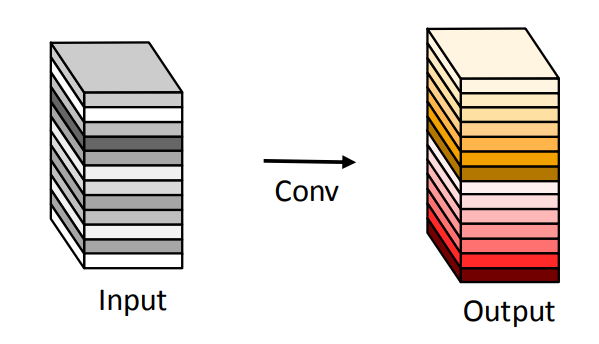
\includegraphics[width = 0.5\textwidth]{传统卷积.png}
    \caption{传统卷积示意图}
    \label{conv}
\end{figure}

如图\ref{identical}所示,每次卷积的所有输出中,可以找到一些相互之间相似度较高的特征图。设图中的A, A’、B B’相似度较高,可以设计一种计算方法替代生成A’和B’的卷积运算,从而达到减小计算量的目的。

\begin{figure}[htbp]
    \centering
    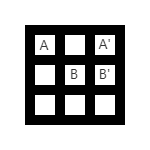
\includegraphics[width = 0.5\textwidth]{重复特征图.png}
    \caption{重复特征图示意图}
    \label{identical}
\end{figure}

\begin{figure}[htbp]
    \centering
    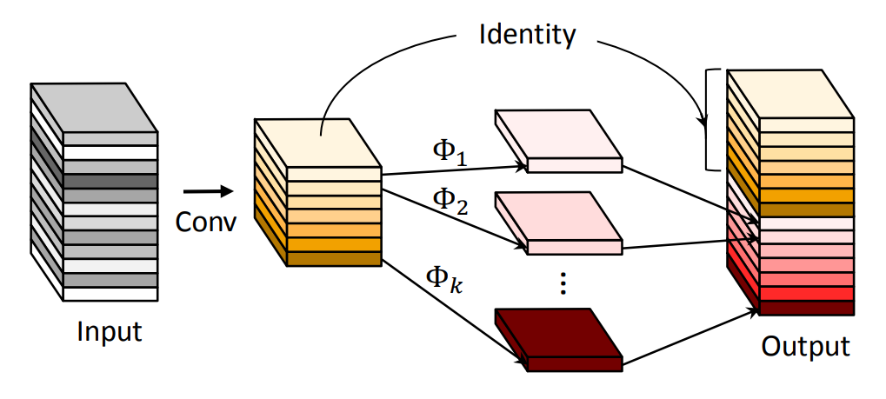
\includegraphics[width = 0.9\textwidth]{ghost卷积.png}
    \caption{ghost卷积示意图}
    \label{ghost1}
\end{figure}

如图\ref{ghost1}所示,ghost模块的做法是用一些更小的卷积核(即参数更少运算更快)替代原先的卷积部分,但是这部分卷积核产生的输出量只能达到相当于本来卷积输出量的一部分,这时根据上文对相似特征图的分析,可以采用一些线性变换的方式去生成剩下的特征图,从而达到用更轻量的卷积滤波器去生成相同规模特征图的目的。

\subsection{基于ghost模块的模型轻量化算法实现}

\begin{figure}[htbp]
    \centering
    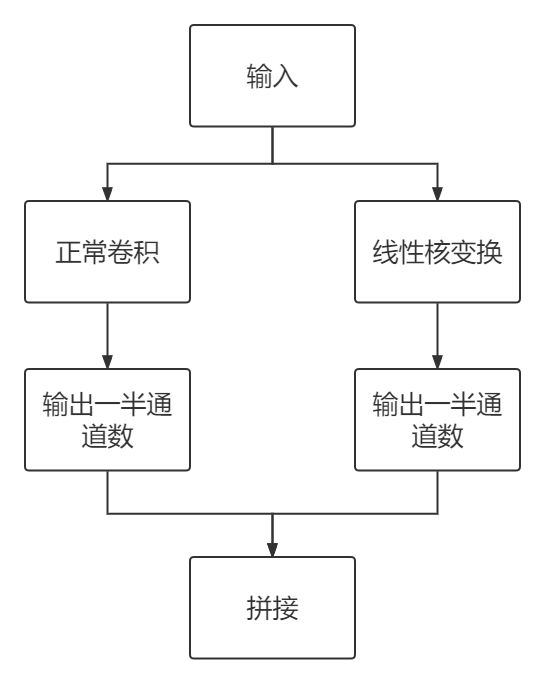
\includegraphics[width = 0.6\textwidth]{ghost算法实现.png}
    \caption{ghost算法实现示意图}
    \label{ghost2}
\end{figure}

本课题的ghost实现流程如图\ref{ghost2}所示,将原始卷积层改变成两部分,分别产生相当于原始卷积层一半通道数的输出(实际上二者的输出比例可以任意调节),可以使得改进后的模块参数量减少。

具体地,本文在实现ghost模块时采用的简单线性变换是分组卷积。图\ref{convp}表示了普通卷积模块的卷积过程,而图\ref{ghostp}表示本文实现的ghost模块的卷积过程。从图\ref{convp}中可以看出,普通卷积的一个卷积核对应一个输出通道,每个卷积核和所有输入通道进行运算;而在图\ref{ghostp}中,首先对输入通道$C1$应用普通卷积,产生$\frac{C2}{2}$个输出特征图,此后应用分组个数为$\frac{C2}{2}$的分组卷积,每个分组内的卷积核不与组外的输入特征图进行运算,分组卷积再产生$\frac{C2}{2}$个输出特征图,因此可以实现ghost模块的输出特征图和普通卷积的输出特征图维度相同。
\begin{figure}[htbp]
    \centering
    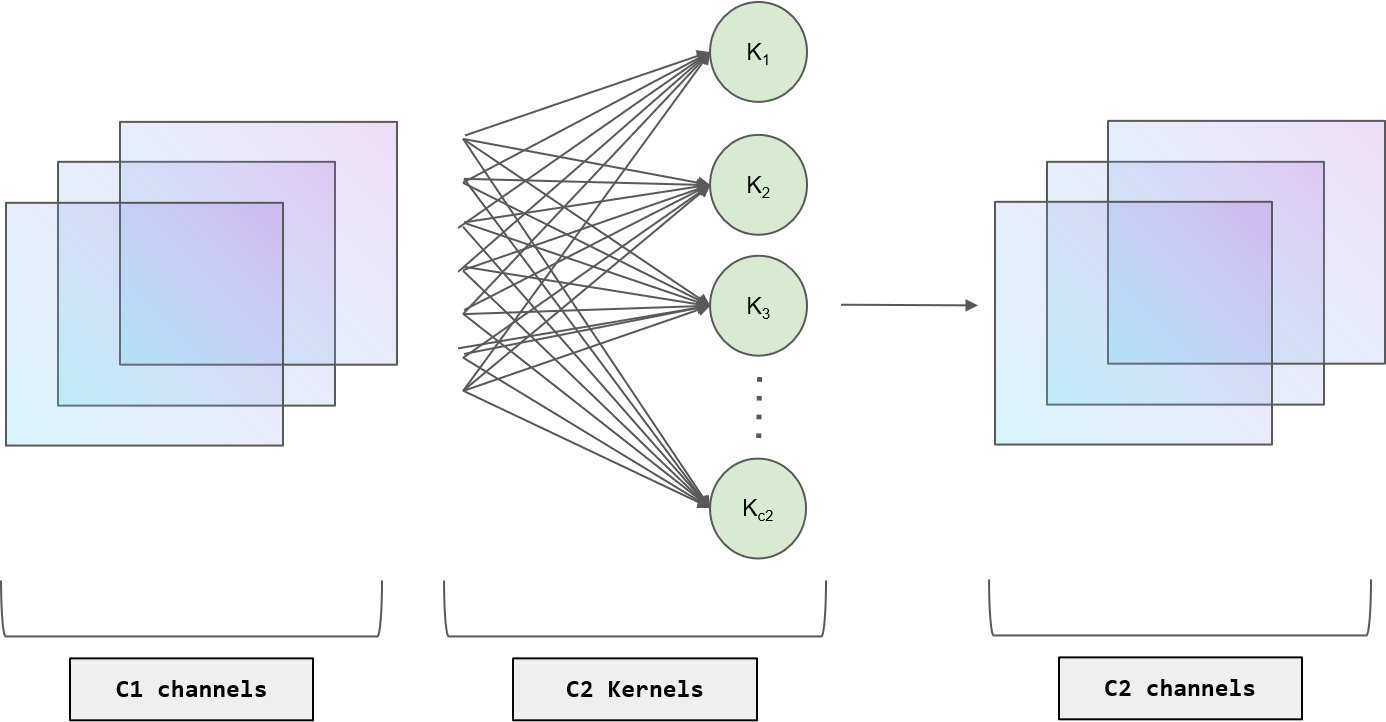
\includegraphics[width = 0.8\textwidth]{普通卷积过程.png}
    \caption{普通卷积实现示意图}
    \label{convp}
\end{figure}

\begin{figure}[htbp]
    \centering
    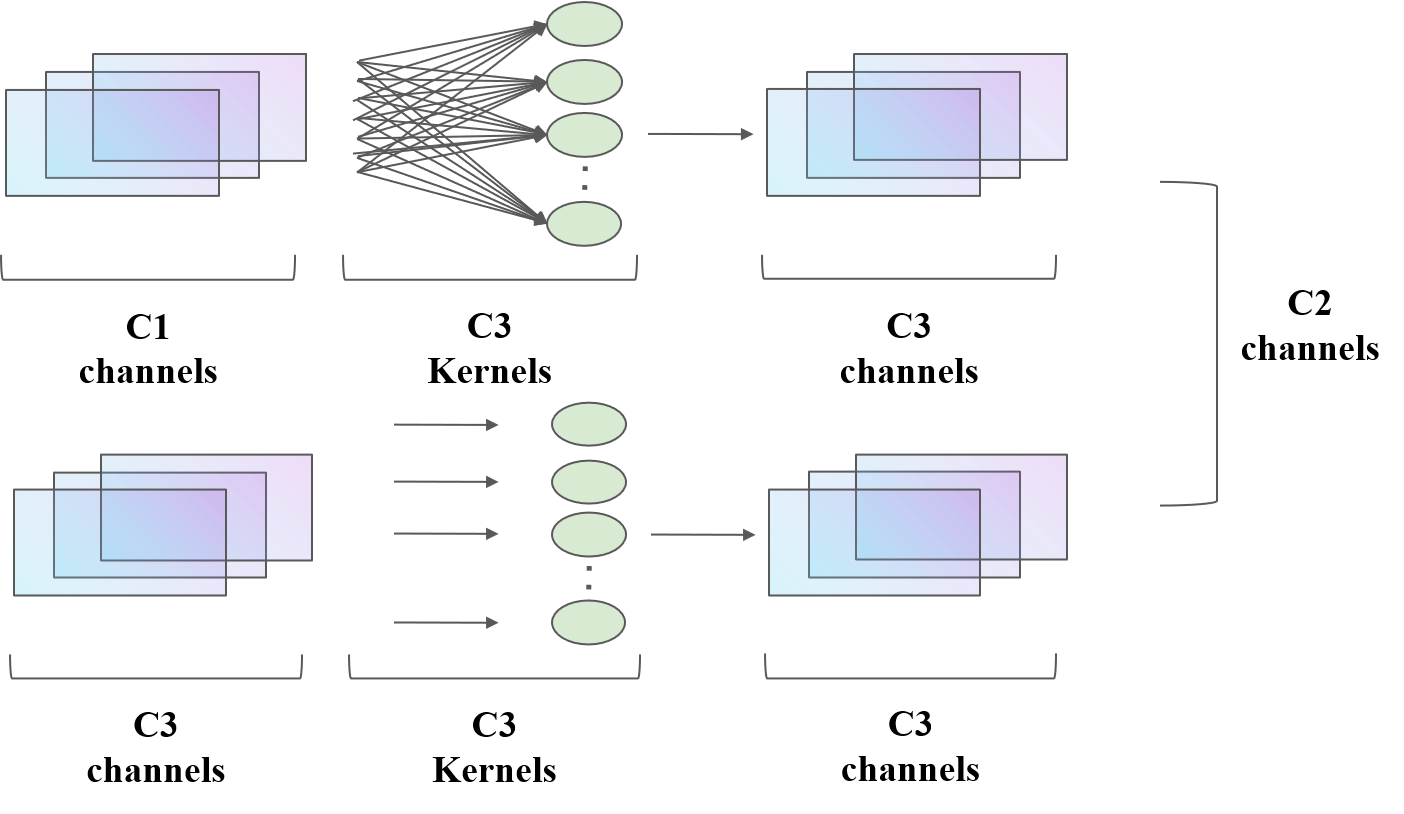
\includegraphics[width = 0.8\textwidth]{ghost卷积过程.png}
    \caption{ghost卷积实现示意图}
    \label{ghostp}
\end{figure}

\begin{figure}[htbp]
	\centering
	\begin{minipage}{0.49\linewidth}
		\centering
		\includegraphics[width=0.9\linewidth]{convfmap.PNG}
		\caption{普通卷积特征图}
		\label{convf}%文中引用该图片代号
	\end{minipage}
	%\qquad
	\begin{minipage}{0.49\linewidth}
		\centering
		\includegraphics[width=0.9\linewidth]{ghostfmap.PNG}
		\caption{ghost卷积特征图}
		\label{ghostf}%文中引用该图片代号
	\end{minipage}
\end{figure}

普通卷积和ghost卷积产生的特征图如图\ref{convf}和图\ref{ghostf}所示,从图中可以看出,由于ghost卷积相当于对普通卷积进行了一定程度的转化,所以ghost卷积产生的特征图和普通卷积产生的特征图存在一定的差别,不过图\ref{convf}和图\ref{ghostf}中确实有相当大比例的对应位置特征图是相似的,这也验证了上文的理论分析。此外,由于ghost卷积减少了网络结构中的参数,所以在简化运算、加速推理的同时,各特征图之间的差异更小,也就是ghost卷积产生的特征图在一定程度上丢失了多样性,也将导致整个网络失去一些特征,降低最终目标检测的精度。

\subsection{ghost算法理论分析}
对于特定的网络结构,在将传统卷积模块替换成ghost卷积模块之后,可以对网络模型的参数数量和推理速度进行理论计算,得出改进后网络相对于原网络的推理加速比和参数压缩比。

(1)相对于普通卷积模块的加速比

\begin{equation}
    \begin{aligned}
    r_{s} &=\frac{n \cdot h^{\prime} \cdot w^{\prime} \cdot c \cdot k \cdot k}{\frac{n}{s} \cdot h^{\prime} \cdot w^{\prime} \cdot c \cdot k \cdot k+(s-1) \cdot \frac{n}{s} \cdot h^{\prime} \cdot w^{\prime} \cdot d \cdot d} \\
    &=\frac{c \cdot k \cdot k}{\frac{1}{s} \cdot c \cdot k \cdot k+\frac{s-1}{s} \cdot d \cdot d} \approx \frac{s \cdot c}{s+c-1} \approx S
    \end{aligned}
    \label{jsb}
\end{equation}

如式\ref{jsb}所示,设输入通道数为$c$,输出通道数为$n$,输入图像高度为$h^{\prime}$和$w^{\prime}$,其中保留的原始卷积通道数为本来的$1/s$,原始卷积核大小为$k*k$,线性核大小为$d*d$,由于线性变换是在每个通道上进行,所以代表线性变换的一项中不含输入通道数$c$。

由式\ref{jsb}可得,将原始卷积模块替换为一半卷积一半线性变换的ghost模块后(即将$s=2$代入),可以得到该模块的理论提速比为2。

(1)相对于普通卷积模块的参数压缩比

\begin{equation}
    r_{c}=\frac{n \cdot c \cdot k \cdot k}{\frac{n}{s} \cdot c \cdot k \cdot k+(s-1) \cdot \frac{n}{s} \cdot d \cdot d} \approx \frac{s \cdot c}{s+c-1} \approx \frac{s c}{c}=S
    \label{csys}
\end{equation}

如式\ref{csys}所示,经过计算可以得到改进后的ghost模块和改进之前的普通卷积模块理论参数压缩比为2。

\subsection{ghost算法实验对比分析}
将ghost模块对应改动部署到YOLOv5网络之后,在实验平台上进行测试验证。分别用YOLOv5网络模型和调整深度之后得到的小型网络(记为YOLOv5s)作为参照,验证YOLOv5+ghost在红外无人机图像数据集上的效果。

\section{轻量化红外无人机目标检测算法嵌入式实现与验证}
为了进一步验证本文提出的轻量化红外无人机目标检测算法的有效性,本节将本文提出的完整算法模型进行转换,并且在嵌入式设备上进行检测和验证。

\subsection{嵌入式设备介绍}
为了满足实际检测任务的需要,本章将本文提到的算法在常用于深度的嵌入式设备 NVIDIA
Jetson AGX Xavier 上进行算法测试,验证算法在实际使用中是否能达到实时性要求。
NVIDIA Jetson AGX Xavier 开发板是英伟达公司推出的嵌入式 AI 超级计算平台,可以
部署在无人机或机器人等诸多终端上,解决移动终端算力不足的局限。NVIDIA
Jetson TX2 采用 Tegra 处理器,内存为 8GB,采用了全新 Pascal 架构 GPU 核心,
更加适合进行一些基于深度学习的计算机视觉任务的开发,具体参数如表\ref{t1}中所
示。NVIDIA Jetson AGX Xavier 具有 MAX Q 和 MAX P 两种运行模式,由于其体型小巧,
性能高效,因此应用场景广泛,如无人机和智能机器人等相关的智能机器领域,
安防和智慧城市等领域。NVIDIA Jetson AGX Xavier 平台出厂自带 Ubuntu 16.04 操作系
统,支持 NVIDIA Jetpack SDK,包括深度学习库、计算机视觉、GPU 计算等功
能,支持下载安装所有台式机所能安装的软件如 Python、Pytorch、TensorFlow
等,轻松配置台式机一样的运行环境。NVIDIA Jetson AGX Xavier 有非常多功能的接口,
比如可以使用 HDMI 接口连接显示器,使用 USB3.0 接口连接摄像头进行实时获
取视频数据用来进行检测或跟踪任务。NVIDIA Jetson AGX Xavier 嵌入式开发平台如图
\ref{agx}所示。近年来由于 TX2 嵌入式平台外形小巧便于集成到各种终端产品中,嵌
入式智能计算平台发展迅猛,但经过实际测试表明嵌入式设备因为 CPU 和 GPU
计算能力与台式机相比仍具有一定差距,TX2 与台式机在相同参数情况下进行相
同的实验时,二者 GPU 运算效率相差将近 10 倍。由于人工智能的兴起,未来嵌
入式设备会向着更加小型化、功耗更低、运行速度更快的方向发展。

\begin{figure}[htbp]
    \centering
    \includegraphics[width = 0.5\textwidth]{agx.jpg}
    \caption{NVIDIA Jetson AGX Xavier实物图}
    \label{agx}
\end{figure}

\begin{table}[htbp]
    \caption{NVIDIA Jetson AGX Xavier参数规格}
    \vspace{0.5em}\centering\wuhao
    \begin{tabular}{cc}
    \toprule
    项目 & 规格\\
    \midrule
    GPU & 512核 NVIDIA Volta GPU,64 Tensor核\\
    CPU & 8核 ARM v8.2 64-bit CPU, 8MB L2 + 4MB L3\\
    DL Accelerator & 2x NVDLA\\
    Vision Accelerator & 2x PVA\\
    Memory & 32GB 256-bit LPDDR4x\\
    Storage & 32GB eMMC 5.1\\
    CSI Camera & 16 lanes MIPI CSI-2\\
    PCIe & x16 connector with x8 PCIe Gen4 or x8 SLVS-EC\\
    Networking & RJ45 (Gigabit Ethernet)\\
    尺寸 & 105mm x 105mm x 65mm\\
    \bottomrule
    \end{tabular}
    \label{t1}
\end{table}

\subsection{ONNX框架}
现如今,各大主流深度学习框架都有着自己独有的特点与魅力,吸引着广大科研与开发人员,例如:
(1)Caffe2:方便机器学习算法和模型大规模部署在移动设备。

(2)PyTorch:PyTorch是一个快速便于实验深度学习框架。但是由于其高度封装,导致部分function不够灵活。

(3)TensorFlow:TensorFlow 是一个开放源代码软件库,是很多主流框架的基础或者依赖。几乎能满足所有机器学习开发的功能,但是也有由于其功能代码过于底层,学习成本高,代码冗繁,编程逻辑与常规不同等缺点。

此外还有:Cognitive Toolkit (CNTK),Apache MXNet,Chainer,Apple CoreML,SciKit-Learn,ML.NET

深度学习算法大多通过计算数据流图来完成神经网络的深度学习过程。 一些框架(例如CNTK,Caffe2,Theano和TensorFlow)使用静态图形,而其他框架(例如PyTorch和Chainer)使用动态图形。 但是这些框架都提供了接口,使开发人员可以轻松构建计算图和运行时,以优化的方式处理图。 这些图用作中间表示(IR),捕获开发人员源代码的特定意图,有助于优化和转换在特定设备(CPU,GPU,FPGA等)上运行。

对于本课题的红外无人机目标检测的任务场景,模型的移动设备部署需要借助tensorrt模型来进行实现,这时候如果把整个模型再重新采用tensorrt进行搭建和训练,无疑是消耗大量的时间和精力。这时就可以用ONNX这样的中间框架来进行已训练模型的转换。

开放式神经网络交换(ONNX)是迈向开放式生态系统的第一步,它使AI开发人员能够随着项目的发展选择合适的工具。 ONNX为AI模型提供开源格式。 它定义了可扩展的计算图模型,以及内置运算符和标准数据类型的定义。 最初的ONNX专注于推理(评估)所需的功能。 ONNX解释计算图的可移植,它使用graph的序列化格式。 它不一定是框架选择在内部使用和操作计算的形式。 例如,如果在优化过程中操作更有效,则实现可以在存储器中以不同方式表示模型。

\subsection{tensorrt框架}
TensorRT 是 NVIDIA 推出的一个高性能的深度学习推理框架,可以让深度学习模型在 NVIDIA GPU 上实现低延迟,高吞吐量的部署。TensorRT 支持 Caffe,TensorFlow,Mxnet,Pytorch 等主流深度学习框架。TensorRT 是一个 C++ 库,并且提供了 C++ API 和 Python API,主要在 NVIDIA GPU 进行高性能的推理 (Inference) 加速。

\subsection{嵌入式平台算法实现及分析}
本节将第三章中研究的基于深度学习的红外无人机目标检测算法进行转换后的算法模型在 NVIDIA AGX XAVIER平台上进行推理测试。算法在嵌入式平台上的检测效果如图\ref{}所示。经过测试,本文提出的算法经过轻量化后在NVIDIA AGX XAVIER平台上的推理时间为36ms,运行速度为28FPS,在保证精度较高的前提下,基本满足实时检测的要求。

\section{本章小结}
本章目的在于将无人机目标检测算法移植到嵌入式平台NVIDIA AGX XAVIER上实现实时检
测。首先介绍了深度学习网络模型轻量化的常用方法,并且选择了一种目标检测领域性能较好的方法即ghost模块替代法。然后用ghost卷积对第三章的算法模型进行压缩,通过在PC平台和在嵌入式平台NVIDIA AGX XAVIER上的测试,证明了本文提出的算法能在红外无人机目标数据集上取得较高的检测精度,并且该算法的轻量化版本能在嵌入式平台上在占用较小内存空间的同时基本实现实时检测。


\backmatter
% !Mode:: "TeX:UTF-8" 
\begin{conclusions}

本文提出了一种基于深度学习的算法来完成红外图像无人机目标检测任务。对比目前已有的目标检测算法,本文提出的检测算法,在红外无人机目标数据集上能取得更高的检测精度并且具备更快的推理速度,本文提出的检测算法可以在嵌入式设备上运行,并且检测速度基本达到了实时推理的要求。

本文所做的工作和取得的主要结果如下:

(1)由于目前开源的红外无人机数据集匮乏,因此本文标注并制作了一套红外无人机数据集。

(2)由于红外图像普遍都存在目标边缘模糊、分辨率低等特点,目前主流的目标检测
算法在红外图像上的检测精度不高,因此在红外
图像的输入到网络进行训练之前需要对红外图像进行数据增强。本文研究了常用的图像增强算法,提出了一种基于通道填充的红外图像数据增强算法,该算
法将原始图像和两个增强过的图像合成BGR三通道输出最终的增强图像,并作为增强数据输入到网络中进行训练。在本文自建红外无人机数据集上的测试结果表明这一数据增强方法提升了算法的检测精度。

(3)由于红外图像无人机目标检测中小目标的出现频率较高,因此一般的算法会因为对小目标检测能力较差而无法胜任红外无人机检测任务。本文针对这一问题设计了基于图像拼接的数据增强算法,将4张原始图像进行拼接后合成新图像输入网络进行训练,增强网络对小目标的检测能力和对复杂背景的辨别能力。在本文自建红外无人机数据集上的测试结果表明这一数据增强方法在结合网络结构的改进后,可以提升算法的检测精度。

(4)针对红外无人机目标检测任务中,小目标出现频率较高,使得目标检测算法容易存在定位不准的问题,从YOLOv5模型的损失函数着手进行改进,设计 GIoU 损失函数代替原来的
IoU损失函数。在本文自建红外无人机数据集上的测试结果表明这一改进可以提升算法的检测精度


(5)本文将研究得到的红外无人机检测算法进行了轻量化,并且在嵌入式设备上进行了算法功能的验证。本文针对嵌入式设备算力有限、检测任务对时间较敏感等问题,基于ghost网络模块对本文提出的红外无人机目标检测算法进行了轻量化,并且将算法的网络模型进行了转换,最终在NVIDIA AGX XAVIER平台上进行了算法的实现。轻量化后的目标检测算法在PC平台上测试了检测精度和推理时间,结果是检测精度略有降低的同时,轻量化算法的推理时间大幅降低。在嵌入式平台上的验证结果表示,本文提出的轻量化红外无人机目标检测算法能基本实现实时检测。

本人在研究生期间在基于深度学习的红外无人机目标检测方面进行了一系列的探
索,既有针对PC场景的算法优化,也有针对嵌入式场景的算法轻量化和嵌入式验证,取得了一定的研究成果。但仍然存在一些需要进
一步改进的地方。后续可以从以下几个方向进行深入研究:

(1)本文建立的数据集中只包含1类无人机目标,后续研究中可以建立更完善的无人机目标数据集,丰富目标的种类。

(2)本文提出的数据增强算法,默认是对于所有的原始图像都进行增强,并且实际增强的算法参数都没有进一步实验,因此该算法还有一定的改进空间,后续可以对这个方向进行继续研究。

(3)本文的算法在NVIDIA AGX XAVIER平台上进行了验证,该平台高度封装且成本较高,因此可能并不完全符合实际检测任务的要求,因此本文的算法有待算力更低且成本较低的嵌入式设备进一步验证。此外,本文的算法嵌入式设备推理速度为30FPS左右,还有进一步提升的空间,并且本文并没有针对硬件设备进行针对性的效率优化,后续可以在这个方向上进行研究。



\end{conclusions}
   % 结论
\bibliographystyle{gbt7714-numerical}
%\bibliographystyle{hithesis} %理论上2020最新要求文献样式GB/T 7714—2015,但若院系要求文献英文作者不全大写,可改用hithesis文献样式
%%%%%%%%%%%%%%%%%%%%%%%%%%%%%%%%%%%%%%%%%%%%%%%%%%%%%%%%%%%%%%%%%%%%%%%%%%%%%%%%
%-- 注意:以下本硕博、博后书序不一致 --%
%%%%%%%%%%%%%%%%%%%%%%%%%%%%%%%%%%%%%%%%%%%%%%%%%%%%%%%%%%%%%%%%%%%%%%%%%%%%%%%%
% 本科书序(哈尔滨、深圳校区)
%%%%%%%%%%%%%%%%%%%%%%%%%%%%%%%%%%%%%%%%%%%%%%%%%%%%%%%%%%%%%%%%%%%%%%%%%%%%%%%%
% \bibliography{reference} % 参考文献
% \authorization %授权
% \authorization[scan.pdf] %添加扫描页的命令,与上互斥
% % !Mode:: "TeX:UTF-8"
\begin{acknowledgements}
转眼两年的研究生生活已近尾声,随着毕业论文的逐渐完成,我的毕业设计将要画上句号。坦白地说,我的毕业设计课题对我来说难度不小,很多地方我都是需要别人的帮助才能完成。因此,在完成毕业设计之后,我真心地向对我提供帮助的人们表示感谢。

首先,我要感谢我的导师吴少川老师。不论是有问题需要讨论,还是文章需要修改,还是学习生活中遇到困难,吴老师总是第一时间不厌其烦地对我提供指导和帮助。在我遇到困难的时候,吴老师总是会为我提供支持和鼓励。我在毕业设计的过程中暴露出很多的问题,吴老师也是及时发现我的问题,并且循循善诱地帮助我解决问题、提高自己。

我还要感谢实验室的老师们和师兄师姐们。感谢他们在我毕设遇到困难的时候对我提供的热情帮助。经过他们的帮助之后,我一步一步地加深对毕业设计课题的理解,才能最终完成毕设的目标。

除此之外,我还要对我的同学们表示真诚的感谢。我在学习和生活中有很多的缺点和问题,因此,不只是毕业设计,在整个硕士研究生生涯中,我都要感谢同学们的陪伴和帮助。和我的同学们共同走过两年,我感受到了真正的快乐和充实,风平浪静时有人分享快乐,荆棘满地时有人并肩前行。感谢我的同学们给我带来人生中快乐的一段时光,感谢他们在我的身边发光发热,我希望毕业后不论是时隔多久,我们的友谊永不褪色。

我要感谢我的老友们。人生短短几十年,能得几人交心,便是一大幸事。在我的硕士研究生生涯里,或者是毕设过程中,或者是之前的若干年,或者是从现在到未来,我的好友们一直都在。感谢他们,可能初见时存在种种的冷漠、滑稽、尴尬、愤怒,不论开场如何,感谢他们走进了我的世界。有了他们的陪伴,我不论遇到什么困难,都能向他们倾诉,向他们寻求帮助,更重要的是,他们给予我力量。
最后,我一定要感谢我的父母。在我成长的过程中,没有一分一秒离得开他们的帮助,在毕设过程中更是如此。感谢我的父母,感谢他们给我的关爱。

非常感谢我的室友刘冠辰给我的大力支持。

\end{acknowledgements}
 %致谢
% \begin{appendix}%附录
% \input{back/appendix01}%本科生翻译论文
% \end{appendix}
%%%%%%%%%%%%%%%%%%%%%%%%%%%%%%%%%%%%%%%%%%%%%%%%%%%%%%%%%%%%%%%%%%%%%%%%%%%%%%%%
% 本科书序(威海校区)
%%%%%%%%%%%%%%%%%%%%%%%%%%%%%%%%%%%%%%%%%%%%%%%%%%%%%%%%%%%%%%%%%%%%%%%%%%%%%%%%
% \authorization %授权
% % \authorization[scan.pdf] %添加扫描页的命令,与上互斥
% \bibliography{reference} % 参考文献
% % !Mode:: "TeX:UTF-8"
\begin{acknowledgements}
转眼两年的研究生生活已近尾声,随着毕业论文的逐渐完成,我的毕业设计将要画上句号。坦白地说,我的毕业设计课题对我来说难度不小,很多地方我都是需要别人的帮助才能完成。因此,在完成毕业设计之后,我真心地向对我提供帮助的人们表示感谢。

首先,我要感谢我的导师吴少川老师。不论是有问题需要讨论,还是文章需要修改,还是学习生活中遇到困难,吴老师总是第一时间不厌其烦地对我提供指导和帮助。在我遇到困难的时候,吴老师总是会为我提供支持和鼓励。我在毕业设计的过程中暴露出很多的问题,吴老师也是及时发现我的问题,并且循循善诱地帮助我解决问题、提高自己。

我还要感谢实验室的老师们和师兄师姐们。感谢他们在我毕设遇到困难的时候对我提供的热情帮助。经过他们的帮助之后,我一步一步地加深对毕业设计课题的理解,才能最终完成毕设的目标。

除此之外,我还要对我的同学们表示真诚的感谢。我在学习和生活中有很多的缺点和问题,因此,不只是毕业设计,在整个硕士研究生生涯中,我都要感谢同学们的陪伴和帮助。和我的同学们共同走过两年,我感受到了真正的快乐和充实,风平浪静时有人分享快乐,荆棘满地时有人并肩前行。感谢我的同学们给我带来人生中快乐的一段时光,感谢他们在我的身边发光发热,我希望毕业后不论是时隔多久,我们的友谊永不褪色。

我要感谢我的老友们。人生短短几十年,能得几人交心,便是一大幸事。在我的硕士研究生生涯里,或者是毕设过程中,或者是之前的若干年,或者是从现在到未来,我的好友们一直都在。感谢他们,可能初见时存在种种的冷漠、滑稽、尴尬、愤怒,不论开场如何,感谢他们走进了我的世界。有了他们的陪伴,我不论遇到什么困难,都能向他们倾诉,向他们寻求帮助,更重要的是,他们给予我力量。
最后,我一定要感谢我的父母。在我成长的过程中,没有一分一秒离得开他们的帮助,在毕设过程中更是如此。感谢我的父母,感谢他们给我的关爱。

非常感谢我的室友刘冠辰给我的大力支持。

\end{acknowledgements}
 %致谢
% \begin{appendix}%附录
% \input{back/appendix01}%本科生翻译论文
% \end{appendix}
%%%%%%%%%%%%%%%%%%%%%%%%%%%%%%%%%%%%%%%%%%%%%%%%%%%%%%%%%%%%%%%%%%%%%%%%%%%%%%%%
% 硕博书序
%%%%%%%%%%%%%%%%%%%%%%%%%%%%%%%%%%%%%%%%%%%%%%%%%%%%%%%%%%%%%%%%%%%%%%%%%%%%%%%%
\bibliography{reference} % 参考文献
\begin{appendix}%附录
\input{back/appA.tex}
\end{appendix}
% !Mode:: "TeX:UTF-8" 
\begin{publication}
\noindent\textbf{发表的相关论文}
\begin{publist}
\item	无

\end{publist}

\noindent\textbf{(三)参与的科研项目及获奖情况}
\begin{publist}
\item	哈工大电信学院第二届”巴龙杯“学术论坛暨研究生创新创意大赛三等奖

\end{publist}
%\vfill
%\hangafter=1\hangindent=2em\noindent
%\setlength{\parindent}{2em}
\end{publication}
    % 所发文章
\include{back/ceindex}    % 索引, 根据自己的情况添加或者不添加,选择自动添加或者手工添加。
\authorization %授权
%\authorization[scan.pdf] %添加扫描页的命令,与上互斥
% !Mode:: "TeX:UTF-8"
\begin{acknowledgements}
转眼两年的研究生生活已近尾声,随着毕业论文的逐渐完成,我的毕业设计将要画上句号。坦白地说,我的毕业设计课题对我来说难度不小,很多地方我都是需要别人的帮助才能完成。因此,在完成毕业设计之后,我真心地向对我提供帮助的人们表示感谢。

首先,我要感谢我的导师吴少川老师。不论是有问题需要讨论,还是文章需要修改,还是学习生活中遇到困难,吴老师总是第一时间不厌其烦地对我提供指导和帮助。在我遇到困难的时候,吴老师总是会为我提供支持和鼓励。我在毕业设计的过程中暴露出很多的问题,吴老师也是及时发现我的问题,并且循循善诱地帮助我解决问题、提高自己。

我还要感谢实验室的老师们和师兄师姐们。感谢他们在我毕设遇到困难的时候对我提供的热情帮助。经过他们的帮助之后,我一步一步地加深对毕业设计课题的理解,才能最终完成毕设的目标。

除此之外,我还要对我的同学们表示真诚的感谢。我在学习和生活中有很多的缺点和问题,因此,不只是毕业设计,在整个硕士研究生生涯中,我都要感谢同学们的陪伴和帮助。和我的同学们共同走过两年,我感受到了真正的快乐和充实,风平浪静时有人分享快乐,荆棘满地时有人并肩前行。感谢我的同学们给我带来人生中快乐的一段时光,感谢他们在我的身边发光发热,我希望毕业后不论是时隔多久,我们的友谊永不褪色。

我要感谢我的老友们。人生短短几十年,能得几人交心,便是一大幸事。在我的硕士研究生生涯里,或者是毕设过程中,或者是之前的若干年,或者是从现在到未来,我的好友们一直都在。感谢他们,可能初见时存在种种的冷漠、滑稽、尴尬、愤怒,不论开场如何,感谢他们走进了我的世界。有了他们的陪伴,我不论遇到什么困难,都能向他们倾诉,向他们寻求帮助,更重要的是,他们给予我力量。
最后,我一定要感谢我的父母。在我成长的过程中,没有一分一秒离得开他们的帮助,在毕设过程中更是如此。感谢我的父母,感谢他们给我的关爱。

非常感谢我的室友刘冠辰给我的大力支持。

\end{acknowledgements}
 %致谢
\include{back/resume}          % 博士学位论文有个人简介
%%%%%%%%%%%%%%%%%%%%%%%%%%%%%%%%%%%%%%%%%%%%%%%%%%%%%%%%%%%%%%%%%%%%%%%%%%%%%%%%
% 博后书序
%%%%%%%%%%%%%%%%%%%%%%%%%%%%%%%%%%%%%%%%%%%%%%%%%%%%%%%%%%%%%%%%%%%%%%%%%%%%%%%%
% \bibliography{reference} % 参考文献
% % !Mode:: "TeX:UTF-8"
\begin{acknowledgements}
转眼两年的研究生生活已近尾声,随着毕业论文的逐渐完成,我的毕业设计将要画上句号。坦白地说,我的毕业设计课题对我来说难度不小,很多地方我都是需要别人的帮助才能完成。因此,在完成毕业设计之后,我真心地向对我提供帮助的人们表示感谢。

首先,我要感谢我的导师吴少川老师。不论是有问题需要讨论,还是文章需要修改,还是学习生活中遇到困难,吴老师总是第一时间不厌其烦地对我提供指导和帮助。在我遇到困难的时候,吴老师总是会为我提供支持和鼓励。我在毕业设计的过程中暴露出很多的问题,吴老师也是及时发现我的问题,并且循循善诱地帮助我解决问题、提高自己。

我还要感谢实验室的老师们和师兄师姐们。感谢他们在我毕设遇到困难的时候对我提供的热情帮助。经过他们的帮助之后,我一步一步地加深对毕业设计课题的理解,才能最终完成毕设的目标。

除此之外,我还要对我的同学们表示真诚的感谢。我在学习和生活中有很多的缺点和问题,因此,不只是毕业设计,在整个硕士研究生生涯中,我都要感谢同学们的陪伴和帮助。和我的同学们共同走过两年,我感受到了真正的快乐和充实,风平浪静时有人分享快乐,荆棘满地时有人并肩前行。感谢我的同学们给我带来人生中快乐的一段时光,感谢他们在我的身边发光发热,我希望毕业后不论是时隔多久,我们的友谊永不褪色。

我要感谢我的老友们。人生短短几十年,能得几人交心,便是一大幸事。在我的硕士研究生生涯里,或者是毕设过程中,或者是之前的若干年,或者是从现在到未来,我的好友们一直都在。感谢他们,可能初见时存在种种的冷漠、滑稽、尴尬、愤怒,不论开场如何,感谢他们走进了我的世界。有了他们的陪伴,我不论遇到什么困难,都能向他们倾诉,向他们寻求帮助,更重要的是,他们给予我力量。
最后,我一定要感谢我的父母。在我成长的过程中,没有一分一秒离得开他们的帮助,在毕设过程中更是如此。感谢我的父母,感谢他们给我的关爱。

非常感谢我的室友刘冠辰给我的大力支持。

\end{acknowledgements}
 %致谢
% \include{back/doctorpublications}    % 所发文章
% % !Mode:: "TeX:UTF-8" 
\begin{publication}
\noindent\textbf{发表的相关论文}
\begin{publist}
\item	无

\end{publist}

\noindent\textbf{(三)参与的科研项目及获奖情况}
\begin{publist}
\item	哈工大电信学院第二届”巴龙杯“学术论坛暨研究生创新创意大赛三等奖

\end{publist}
%\vfill
%\hangafter=1\hangindent=2em\noindent
%\setlength{\parindent}{2em}
\end{publication}
    % 所发文章
% \include{back/resume}          % 博士学位论文有个人简介
% \include{back/correspondingaddr} %通信地址
%%%%%%%%%%%%%%%%%%%%%%%%%%%%%%%%%%%%%%%%%%%%%%%%%%%%%%%%%%%%%%%%%%%%%%%%%%%%%%%%
\end{document}
% Local Variables:
% TeX-engine: xetex
% End:
